\chapter{Range-Rename}
\label{chap:rename}

This chapter describes the range-rename operation~\citep{betrfs4,betrfs4tos}
on \bets.
Full-path-indexed \betrfs can implement a file system rename by invoking the
range-rename operation on the \bet that updates all related key in the rename.
For example, renaming ``/foo'' to ``/bar'' invokes a range-rename operation
that updates all keys with prefix ``/foo'' to have prefix ``/bar''.
The goal of this design is to get good locality from full-path indexing
while having good rename performance through an efficient range-rename
implementation.

Section~\ref{sec:rr:int} describes the range-rename interface and shows how
\betrfs can implement file system renames by calling range-rename operations.
Then, Section~\ref{sec:rr:op} discusses how to implement the range-rename operation
in an I/O-efficient way on \bets.
In particular, the range-rename operation introduces two key techniques,
\textbf{tree surgery} (Section~\ref{sec:rr:op:surgery}) and
\textbf{key lifting} (Section~\ref{sec:rr:op:lift}).
Finally, Section~\ref{sec:rr:impl} explains implementation details of
the range-rename operation in \fti and \betrfs.

\section{The range-rename interface}
\label{sec:rr:int}

Range-rename is a new key/value store operation defined as
range-rename(\spre, \dpre).
The range-rename operation takes two prefixes, \spre and \dpre, as arguments
and updates source and destination key/value pairs
(a source/destination key/value pair has the prefix \spre/\dpre in its key).
Range-rename(\spre, \dpre) does three things atomically:
\begin{itemize}
\item the range-rename operation deletes all destination key/value pairs
    from the key/value store
\item then, for each source key/value pair $(k,v)$ in the key/value store,
    the range-rename operation creates a key/value pair $(k',v)$
    in the key/value store, where $k$ is the concatenation of \spre and some
    suffix $s$ and $k'$ is the concatenation of \dpre and the same suffix $s$;
\item at last, the range-rename operation deletes all source key/value pairs
    from the key/value store.
\end{itemize}
In other words, the range-rename deletes all destination key/value pairs and
updates all source key/value pairs, changing the key prefix from \spre to \dpre.

To see how range-rename accomplishes file system renames in full-path-indexed
\betrfs, consider renaming file ``/foo'' to ``/bar''.
In \mdb, \betrfs needs to insert the destination key ``/bar''
(this insert overwrites the old value of ``/bar'', if it exists)
and delete the source key ``/foo'', resulting in two operations on the \bet.
On the other hand, in \ddb, \betrfs needs to delete all data keys of ``/bar''
(POSIX allows file renames to overwrite the destination file) and update all
data keys of ``/foo'' to be data keys of ``/bar''.
The whole work in \ddb can be done by calling range-rename(``/foo'',``/bar'')
(a data key is the concatenation of the full-path and an 8-byte block number).

Similarly, consider renaming directory ``/baz'' to ``/qux''.
In \mdb, \betrfs also needs to insert the destination key ``/qux'' and delete
the source key ``/baz'' with two operations on the \bet.
Additionally, \betrfs needs to update all keys with prefix ``/baz/'' to have
prefix ``/qux/''
(POSIX only allows directory renames to overwrite an empty directory, which
means there cannot be any key with prefix ``/qux/''),
which is handled in range-rename(``/baz/'', ``/qux/'').
Likewise, in \ddb, \betrfs needs to update all keys with prefix ``/baz/''
to have prefix ``/qux/'', which is done by range-rename(``/baz/'', ``/qux/'')
(directory doesn't have any data key).

Also, \betrfs puts all operations in a file system rename in a transaction
so that all changes are committed atomically.

\begin{table}[t]
    \centering
    \begin{tabular}{c | l}
        \hline
        Type of Rename & Key/Value Store Operations \\
        \hline
        \hline
        File Rename & transaction\_begin(); \\
                    & \mdb$\rightarrow$put(\textit{dst}); \\
                    & \mdb$\rightarrow$del(\textit{src}); \\
                    & \ddb$\rightarrow$range-rename(\textit{src}, \textit{dst}); \\
                    & transaction\_end(); \\
        \hline
        Directory Rename & transaction\_begin(); \\
                         & \mdb$\rightarrow$put(\textit{dst}); \\
                         & \mdb$\rightarrow$del(\textit{src}); \\
                         & \mdb$\rightarrow$range-rename(\textit{src/}, \textit{dst/}); \\
                         & \ddb$\rightarrow$range-rename(\textit{src/}, \textit{dst/}); \\
                         & transaction\_end(); \\
        \hline
    \end{tabular}
    \caption[Full-path-indexed \betrfs implements file system renames with range-rename]{\label{tab:fsrr}
        Full-path-indexed \betrfs renames \textit{src} to \textit{dst} by
        invoking range-rename and other operations on \bets in a transaction.}
\end{table}

Table~\ref{tab:fsrr} summarizes how file system renames can be done with
range-rename operations in full-path-index \betrfs.
Briefly speaking, full-path-indexed \betrfs can finish a file rename by
invoking three operations on \bets: an insert, a delete and a range-rename
operation.
And a directory rename can be done with an insert, a delete and two
range-rename operations.

In fact, previous full-path-indexed \betrfs implemented the
range-rename operation with existing \bet operations,
\texttt{del}, \texttt{get} and \texttt{put}.
However, this range-rename implementation updates all source and destination
key/value pairs.
The I/O-cost of this range-rename implementation increases
when the number of source and destination key/value pairs grows.
Efficient file system renames in full-path-indexed \betrfs require an efficient
range-rename implementation, that is, a range-rename implementation that
completes in a bounded number of I/Os
that doesn't grow as the number of related keys grows.

\section{The range-rename operation}
\label{sec:rr:op}

This section describes the range-rename implementation on the
\bet whose cost doesn't grow as the number of related keys grows.
The efficient range-rename operation requires lexicographic key order so that
keys with the same prefix are contiguous in the key space.
With contiguous keys, the range-rename operation can create an isolated subtree,
which contains all keys of a certain prefix in the \bet,
through \textbf{tree surgery}.
Then, the range-rename operation moves the isolated subtree to another location
in the \bet.
The prefixes of keys in the subtree are updated automatically through
\textbf{key lifting}, which transforms \bets into lifted \bets.

Section~\ref{sec:rr:op:surgery} describes tree surgery, which splits nodes in the
\bet to create an isolated subtree of a prefix.
Tree surgery also flushes messages in the \bet to push all related messages into
the isolated subtree.
Then, Section~\ref{sec:rr:op:lift} introduces key lifting, which transforms the
\bets into lifted \bets that update prefixes of keys in a subtree
automatically when the subtree is moved to another location.
At last, Section~\ref{sec:rr:op:rr} combines the two techniques and shows how
to implement the efficient range-rename operation on lifted \bets.

\subsection{Tree surgery}
\label{sec:rr:op:surgery}

\begin{figure}
    \begin{subfigure}{\textwidth}
        \centering
        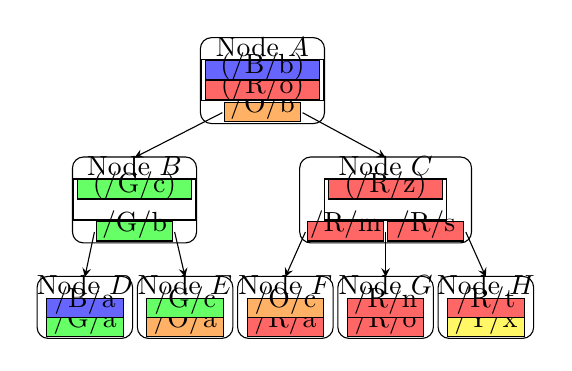
\begin{tikzpicture}
    \node[anchor=south, rectangle, rounded corners, minimum width=.1\textwidth, minimum height=.065\textwidth, draw=black] at (.0\textwidth, 0) {};
    \node[anchor=south] at (.0\textwidth, .036\textwidth) {Node $F$};
    \node[anchor=south, rectangle, minimum width=.08\textwidth, minimum height=.02\textwidth, draw=black, fill={red!60}] at (.0\textwidth, .002\textwidth) {};
    \node[anchor=south] at (.0\textwidth, -0.005\textwidth) {/R/a};
    \node[anchor=south, rectangle, minimum width=.08\textwidth, minimum height=.02\textwidth, draw=black, fill={orange!60}] at (.0\textwidth, .022\textwidth) {};
    \node[anchor=south] at (.0\textwidth, .015\textwidth) {/O/c};

    \node[anchor=south, rectangle, rounded corners, minimum width=.1\textwidth, minimum height=.065\textwidth, draw=black] at (.105\textwidth, 0) {};
    \node[anchor=south] at (.105\textwidth, .036\textwidth) {Node $G$};
    \node[anchor=south, rectangle, minimum width=.08\textwidth, minimum height=.02\textwidth, draw=black, fill={red!60}] at (.105\textwidth, .002\textwidth) {};
    \node[anchor=south] at (.105\textwidth, -0.005\textwidth) {/R/o};
    \node[anchor=south, rectangle, minimum width=.08\textwidth, minimum height=.02\textwidth, draw=black, fill={red!60}] at (.105\textwidth, .022\textwidth) {};
    \node[anchor=south] at (.105\textwidth, .015\textwidth) {/R/n};

    \node[anchor=south, rectangle, rounded corners, minimum width=.1\textwidth, minimum height=.065\textwidth, draw=black] at (.21\textwidth, 0) {};
    \node[anchor=south] at (.21\textwidth, .036\textwidth) {Node $H$};
    \node[anchor=south, rectangle, minimum width=.08\textwidth, minimum height=.02\textwidth, draw=black, fill={yellow!60}] at (.21\textwidth, .002\textwidth) {};
    \node[anchor=south] at (.21\textwidth, -0.005\textwidth) {/Y/x};
    \node[anchor=south, rectangle, minimum width=.08\textwidth, minimum height=.02\textwidth, draw=black, fill={red!60}] at (.21\textwidth, .022\textwidth) {};
    \node[anchor=south] at (.21\textwidth, .015\textwidth) {/R/t};

    \node[anchor=south, rectangle, rounded corners, minimum width=.1\textwidth, minimum height=.065\textwidth, draw=black] at (-.105\textwidth, 0) {};
    \node[anchor=south] at (-.105\textwidth, .036\textwidth) {Node $E$};
    \node[anchor=south, rectangle, minimum width=.08\textwidth, minimum height=.02\textwidth, draw=black, fill={orange!60}] at (-.105\textwidth, .002\textwidth) {};
    \node[anchor=south] at (-.105\textwidth, -0.005\textwidth) {/O/a};
    \node[anchor=south, rectangle, minimum width=.08\textwidth, minimum height=.02\textwidth, draw=black, fill={green!60}] at (-.105\textwidth, .022\textwidth) {};
    \node[anchor=south] at (-.105\textwidth, .015\textwidth) {/G/c};

    \node[anchor=south, rectangle, rounded corners, minimum width=.1\textwidth, minimum height=.065\textwidth, draw=black] at (-.21\textwidth, 0) {};
    \node[anchor=south] at (-.21\textwidth, .036\textwidth) {Node $D$};
    \node[anchor=south, rectangle, minimum width=.08\textwidth, minimum height=.02\textwidth, draw=black, fill={green!60}] at (-.21\textwidth, .002\textwidth) {};
    \node[anchor=south] at (-.21\textwidth, -0.005\textwidth) {/G/a};
    \node[anchor=south, rectangle, minimum width=.08\textwidth, minimum height=.02\textwidth, draw=black, fill={blue!60}] at (-.21\textwidth, .022\textwidth) {};
    \node[anchor=south] at (-.21\textwidth, .015\textwidth) {/B/a};

    \node[anchor=south, rectangle, rounded corners, minimum width=.13\textwidth, minimum height=.09\textwidth, draw=black] at (-.158\textwidth, .1\textwidth) {};
    \node[anchor=south] at (-.158\textwidth, .161\textwidth) {Node $B$};
    \node[anchor=south, rectangle, minimum width=.08\textwidth, minimum height=.02\textwidth, draw=black, fill={green!60}] at (-.158\textwidth, .102\textwidth) {};
    \node[anchor=south] at (-.158\textwidth, .095\textwidth) {/G/b};
    \node[anchor=south, rectangle,minimum width=.128\textwidth, minimum height=.043\textwidth, draw=black] at (-.158\textwidth, .124\textwidth) {};
    \node[anchor=south, rectangle, minimum width=.12\textwidth, minimum height=.02\textwidth, draw=black, fill={green!60}] at (-.158\textwidth, .146\textwidth) {};
    \node[anchor=south] at  (-.158\textwidth, .136\textwidth) {\delm(/G/c)};

    \node[anchor=south, rectangle, rounded corners, minimum width=.18\textwidth, minimum height=.09\textwidth, draw=black] at (.105\textwidth, .1\textwidth) {};
    \node[anchor=south] at (.105\textwidth, .161\textwidth) {Node $C$};
    \node[anchor=south, rectangle, minimum width=.08\textwidth, minimum height=.02\textwidth, draw=black, fill={red!60}] at (.063\textwidth, .102\textwidth) {};
    \node[anchor=south] at (.063\textwidth, .095\textwidth) {/R/m};
    \node[anchor=south, rectangle, minimum width=.08\textwidth, minimum height=.02\textwidth, draw=black, fill={red!60}] at (.147\textwidth, .102\textwidth) {};
    \node[anchor=south] at (.147\textwidth, .095\textwidth) {/R/s};
    \node[anchor=south, rectangle, minimum width=.128\textwidth, minimum height=.043\textwidth, draw=black] at (.105\textwidth, .124\textwidth) {};
    \node[anchor=south, rectangle, minimum width=.12\textwidth, minimum height=.02\textwidth, draw=black, fill={red!60}] at (.105\textwidth, .146\textwidth) {};
    \node[anchor=south] at  (.105\textwidth, .136\textwidth) {\putm(/R/z)};

    \node[anchor=south, rectangle, rounded corners, minimum width=.13\textwidth, minimum height=.09\textwidth, draw=black] at (-.024\textwidth, .225\textwidth) {};
    \node[anchor=south] at (-.024\textwidth, .286\textwidth) {Node $A$};
    \node[anchor=south, rectangle, minimum width=.08\textwidth, minimum height=.02\textwidth, draw=black, fill={orange!60}] at (-.024\textwidth, .227\textwidth) {};
    \node[anchor=south] at (-.024\textwidth, .22\textwidth) {/O/b};
    \node[anchor=south, rectangle, minimum width=.128\textwidth, minimum height=.043\textwidth, draw=black] at (-.024\textwidth, .249\textwidth) {};
    \node[anchor=south, rectangle, minimum width=.12\textwidth, minimum height=.02\textwidth, draw=black, fill={red!60}] at (-.024\textwidth, .25\textwidth) {};
    \node[anchor=south] at  (-.024\textwidth, .24\textwidth) {\delm(/R/o)};
    \node[anchor=south, rectangle, minimum width=.12\textwidth, minimum height=.02\textwidth, draw=black, fill={blue!60}] at (-.024\textwidth, .271\textwidth) {};
    \node[anchor=south] at  (-.024\textwidth, .261\textwidth) {\putm(/B/b)};

    \draw[->, >=stealth] (-.2\textwidth, .112\textwidth) -- (-.21\textwidth, .065\textwidth);
    \draw[->, >=stealth] (-.116\textwidth, .112\textwidth) -- (-.105\textwidth, .065\textwidth);
    \draw[->, >=stealth] (.021\textwidth, .112\textwidth) -- (.0\textwidth, .065\textwidth);
    \draw[->, >=stealth] (.105\textwidth, .112\textwidth) -- (.105\textwidth, .065\textwidth);
    \draw[->, >=stealth] (.189\textwidth, .112\textwidth) -- (.21\textwidth, .065\textwidth);
    \draw[->, >=stealth] (-.066\textwidth, .237\textwidth) -- (-.158\textwidth, .19\textwidth);
    \draw[->, >=stealth] (.018\textwidth, .237\textwidth) -- (.105\textwidth, .19\textwidth);
\end{tikzpicture}

        \caption{\label{subfig:slice-1} The \bet before tree surgery.}
    \end{subfigure}
    \begin{subfigure}{\textwidth}
        \centering
        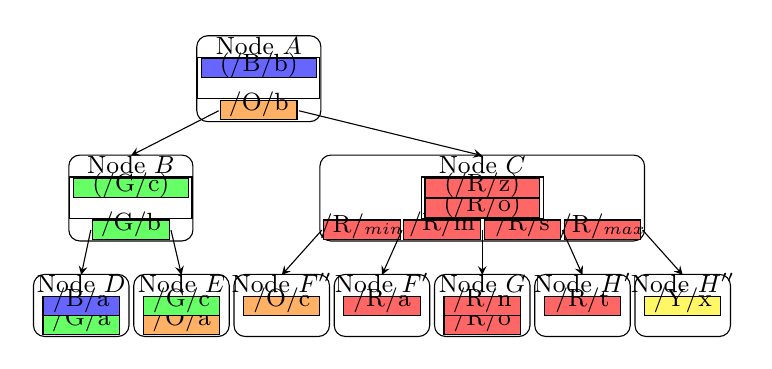
\begin{tikzpicture}
    \node[anchor=south, rectangle, rounded corners, minimum width=.1\textwidth, minimum height=.065\textwidth, draw=black] at (.0\textwidth, 0) {};
    \node[anchor=south, font=\small] at (.0\textwidth, .036\textwidth) {Node $F''$};
    \node[anchor=south, rectangle, minimum width=.08\textwidth, minimum height=.02\textwidth, draw=black, fill={orange!60}] at (.0\textwidth, .022\textwidth) {};
    \node[anchor=south, font=\small] at (.0\textwidth, .015\textwidth) {/O/c};

    \node[anchor=south, rectangle, rounded corners, minimum width=.1\textwidth, minimum height=.065\textwidth, draw=black] at (.105\textwidth, 0) {};
    \node[anchor=south, font=\small] at (.105\textwidth, .036\textwidth) {Node $F'$};
    \node[anchor=south, rectangle, minimum width=.08\textwidth, minimum height=.02\textwidth, draw=black, fill={red!60}] at (.105\textwidth, .022\textwidth) {};
    \node[anchor=south, font=\small] at (.105\textwidth, .015\textwidth) {/R/a};

    \node[anchor=south, rectangle, rounded corners, minimum width=.1\textwidth, minimum height=.065\textwidth, draw=black] at (.21\textwidth, 0) {};
    \node[anchor=south, font=\small] at (.21\textwidth, .036\textwidth) {Node $G$};
    \node[anchor=south, rectangle, minimum width=.08\textwidth, minimum height=.02\textwidth, draw=black, fill={red!60}] at (.21\textwidth, .002\textwidth) {};
    \node[anchor=south, font=\small] at (.21\textwidth, -0.005\textwidth) {/R/o};
    \node[anchor=south, rectangle, minimum width=.08\textwidth, minimum height=.02\textwidth, draw=black, fill={red!60}] at (.21\textwidth, .022\textwidth) {};
    \node[anchor=south, font=\small] at (.21\textwidth, .015\textwidth) {/R/n};

    \node[anchor=south, rectangle, rounded corners, minimum width=.1\textwidth, minimum height=.065\textwidth, draw=black] at (.315\textwidth, 0) {};
    \node[anchor=south, font=\small] at (.315\textwidth, .036\textwidth) {Node $H'$};
    \node[anchor=south, rectangle, minimum width=.08\textwidth, minimum height=.02\textwidth, draw=black, fill={red!60}] at (.315\textwidth, .022\textwidth) {};
    \node[anchor=south, font=\small] at (.315\textwidth, .015\textwidth) {/R/t};

    \node[anchor=south, rectangle, rounded corners, minimum width=.1\textwidth, minimum height=.065\textwidth, draw=black] at (.42\textwidth, 0) {};
    \node[anchor=south, font=\small] at (.42\textwidth, .036\textwidth) {Node $H''$};
    \node[anchor=south, rectangle, minimum width=.08\textwidth, minimum height=.02\textwidth, draw=black, fill={yellow!60}] at (.42\textwidth, .022\textwidth) {};
    \node[anchor=south, font=\small] at (.42\textwidth, .015\textwidth) {/Y/x};

    \node[anchor=south, rectangle, rounded corners, minimum width=.1\textwidth, minimum height=.065\textwidth, draw=black] at (-.105\textwidth, 0) {};
    \node[anchor=south, font=\small] at (-.105\textwidth, .036\textwidth) {Node $E$};
    \node[anchor=south, rectangle, minimum width=.08\textwidth, minimum height=.02\textwidth, draw=black, fill={orange!60}] at (-.105\textwidth, .002\textwidth) {};
    \node[anchor=south, font=\small] at (-.105\textwidth, -0.005\textwidth) {/O/a};
    \node[anchor=south, rectangle, minimum width=.08\textwidth, minimum height=.02\textwidth, draw=black, fill={green!60}] at (-.105\textwidth, .022\textwidth) {};
    \node[anchor=south, font=\small] at (-.105\textwidth, .015\textwidth) {/G/c};

    \node[anchor=south, rectangle, rounded corners, minimum width=.1\textwidth, minimum height=.065\textwidth, draw=black] at (-.21\textwidth, 0) {};
    \node[anchor=south, font=\small] at (-.21\textwidth, .036\textwidth) {Node $D$};
    \node[anchor=south, rectangle, minimum width=.08\textwidth, minimum height=.02\textwidth, draw=black, fill={green!60}] at (-.21\textwidth, .002\textwidth) {};
    \node[anchor=south, font=\small] at (-.21\textwidth, -0.005\textwidth) {/G/a};
    \node[anchor=south, rectangle, minimum width=.08\textwidth, minimum height=.02\textwidth, draw=black, fill={blue!60}] at (-.21\textwidth, .022\textwidth) {};
    \node[anchor=south, font=\small] at (-.21\textwidth, .015\textwidth) {/B/a};

    \node[anchor=south, rectangle, rounded corners, minimum width=.13\textwidth, minimum height=.09\textwidth, draw=black] at (-.158\textwidth, .1\textwidth) {};
    \node[anchor=south, font=\small] at (-.158\textwidth, .161\textwidth) {Node $B$};
    \node[anchor=south, rectangle, minimum width=.08\textwidth, minimum height=.02\textwidth, draw=black, fill={green!60}] at (-.158\textwidth, .102\textwidth) {};
    \node[anchor=south, font=\small] at (-.158\textwidth, .095\textwidth) {/G/b};
    \node[anchor=south, rectangle,minimum width=.128\textwidth, minimum height=.043\textwidth, draw=black] at (-.158\textwidth, .124\textwidth) {};
    \node[anchor=south, rectangle, minimum width=.12\textwidth, minimum height=.02\textwidth, draw=black, fill={green!60}] at (-.158\textwidth, .146\textwidth) {};
    \node[anchor=south, font=\small] at  (-.158\textwidth, .136\textwidth) {\delm(/G/c)};

    \node[anchor=south, rectangle, rounded corners, minimum width=.34\textwidth, minimum height=.09\textwidth, draw=black] at (.21\textwidth, .1\textwidth) {};
    \node[anchor=south, font=\small] at (.21\textwidth, .161\textwidth) {Node $C$};
    \node[anchor=south, rectangle, minimum width=.08\textwidth, minimum height=.02\textwidth, draw=black, fill={red!60}] at (.084\textwidth, .102\textwidth) {};
    \node[anchor=south, font=\small] at (.084\textwidth, .093\textwidth) {/R/$_{min}$};
    \node[anchor=south, rectangle, minimum width=.08\textwidth, minimum height=.02\textwidth, draw=black, fill={red!60}] at (.168\textwidth, .102\textwidth) {};
    \node[anchor=south, font=\small] at (.168\textwidth, .095\textwidth) {/R/m};
    \node[anchor=south, rectangle, minimum width=.08\textwidth, minimum height=.02\textwidth, draw=black, fill={red!60}] at (.252\textwidth, .102\textwidth) {};
    \node[anchor=south, font=\small] at (.252\textwidth, .095\textwidth) {/R/s};
    \node[anchor=south, rectangle, minimum width=.08\textwidth, minimum height=.02\textwidth, draw=black, fill={red!60}] at (.336\textwidth, .102\textwidth) {};
    \node[anchor=south, font=\small] at (.336\textwidth, .093\textwidth) {/R/$_{max}$};
    \node[anchor=south, rectangle, minimum width=.128\textwidth, minimum height=.043\textwidth, draw=black] at (.21\textwidth, .124\textwidth) {};
    \node[anchor=south, rectangle, minimum width=.12\textwidth, minimum height=.02\textwidth, draw=black, fill={red!60}] at (.21\textwidth, .125\textwidth) {};
    \node[anchor=south, font=\small] at  (.21\textwidth, .115\textwidth) {\delm(/R/o)};
    \node[anchor=south, rectangle, minimum width=.12\textwidth, minimum height=.02\textwidth, draw=black, fill={red!60}] at (.21\textwidth, .146\textwidth) {};
    \node[anchor=south, font=\small] at  (.21\textwidth, .136\textwidth) {\putm(/R/z)};

    \node[anchor=south, rectangle, rounded corners, minimum width=.13\textwidth, minimum height=.09\textwidth, draw=black] at (-.024\textwidth, .225\textwidth) {};
    \node[anchor=south, font=\small] at (-.024\textwidth, .286\textwidth) {Node $A$};
    \node[anchor=south, rectangle, minimum width=.08\textwidth, minimum height=.02\textwidth, draw=black, fill={orange!60}] at (-.024\textwidth, .227\textwidth) {};
    \node[anchor=south, font=\small] at (-.024\textwidth, .22\textwidth) {/O/b};
    \node[anchor=south, rectangle, minimum width=.128\textwidth, minimum height=.043\textwidth, draw=black] at (-.024\textwidth, .249\textwidth) {};
    \node[anchor=south, rectangle, minimum width=.12\textwidth, minimum height=.02\textwidth, draw=black, fill={blue!60}] at (-.024\textwidth, .271\textwidth) {};
    \node[anchor=south, font=\small] at  (-.024\textwidth, .261\textwidth) {\putm(/B/b)};

    \draw[->, >=stealth] (-.2\textwidth, .112\textwidth) -- (-.21\textwidth, .065\textwidth);
    \draw[->, >=stealth] (-.116\textwidth, .112\textwidth) -- (-.105\textwidth, .065\textwidth);
    \draw[->, >=stealth] (.042\textwidth, .112\textwidth) -- (.0\textwidth, .065\textwidth);
    \draw[->, >=stealth] (.126\textwidth, .112\textwidth) -- (.105\textwidth, .065\textwidth);
    \draw[->, >=stealth] (.21\textwidth, .112\textwidth) -- (.21\textwidth, .065\textwidth);
    \draw[->, >=stealth] (.294\textwidth, .112\textwidth) -- (.315\textwidth, .065\textwidth);
    \draw[->, >=stealth] (.378\textwidth, .112\textwidth) -- (.42\textwidth, .065\textwidth);
    \draw[->, >=stealth] (-.066\textwidth, .237\textwidth) -- (-.158\textwidth, .19\textwidth);
    \draw[->, >=stealth] (.018\textwidth, .237\textwidth) -- (.21\textwidth, .19\textwidth);
\end{tikzpicture}

        \caption{\label{subfig:slice-2} Tree surgery splits leaf nodes.}
    \end{subfigure}
    \begin{subfigure}{\textwidth}
        \centering
        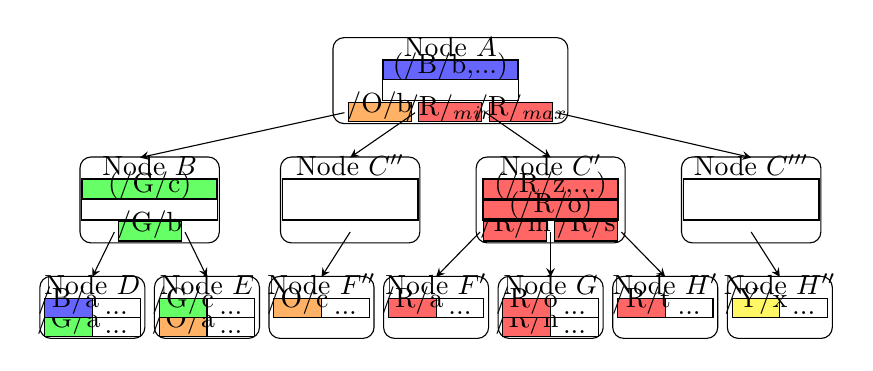
\begin{tikzpicture}
    \node[anchor=south, rectangle, rounded corners, minimum width=.11\textwidth, minimum height=.065\textwidth, draw=black] at (-.005\textwidth, 0) {};
    \node[anchor=south] at (-.005\textwidth, .036\textwidth) {Node $F''$};
    \node[anchor=south, rectangle, minimum width=.05\textwidth, minimum height=.02\textwidth, draw=black, fill={orange!60}] at (-.03\textwidth, .022\textwidth) {};
    \node[anchor=south] at (-.03\textwidth, .015\textwidth) {/O/c};
    \node[anchor=south, rectangle, minimum width=.05\textwidth, minimum height=.02\textwidth, draw=black] at (.02\textwidth, .022\textwidth) {};
    \node[anchor=south] at (.02\textwidth, .015\textwidth) {...};

    \node[anchor=south, rectangle, rounded corners, minimum width=.11\textwidth, minimum height=.065\textwidth, draw=black] at (.115\textwidth, 0) {};
    \node[anchor=south] at (.115\textwidth, .036\textwidth) {Node $F'$};
    \node[anchor=south, rectangle, minimum width=.05\textwidth, minimum height=.02\textwidth, draw=black, fill={red!60}] at (.09\textwidth, .022\textwidth) {};
    \node[anchor=south] at (.09\textwidth, .015\textwidth) {/R/a};
    \node[anchor=south, rectangle, minimum width=.05\textwidth, minimum height=.02\textwidth, draw=black] at (.14\textwidth, .022\textwidth) {};
    \node[anchor=south] at (.14\textwidth, .015\textwidth) {...};

    \node[anchor=south, rectangle, rounded corners, minimum width=.11\textwidth, minimum height=.065\textwidth, draw=black] at (.235\textwidth, 0) {};
    \node[anchor=south] at (.235\textwidth, .036\textwidth) {Node $G$};
    \node[anchor=south, rectangle, minimum width=.05\textwidth, minimum height=.02\textwidth, draw=black, fill={red!60}] at (.21\textwidth, .002\textwidth) {};
    \node[anchor=south] at (.21\textwidth, -0.005\textwidth) {/R/n};
    \node[anchor=south, rectangle, minimum width=.05\textwidth, minimum height=.02\textwidth, draw=black] at (.26\textwidth, .002\textwidth) {};
    \node[anchor=south] at (.26\textwidth, -0.005\textwidth) {...};
    \node[anchor=south, rectangle, minimum width=.05\textwidth, minimum height=.02\textwidth, draw=black, fill={red!60}] at (.21\textwidth, .022\textwidth) {};
    \node[anchor=south] at (.21\textwidth, .015\textwidth) {/R/o};
    \node[anchor=south, rectangle, minimum width=.05\textwidth, minimum height=.02\textwidth, draw=black] at (.26\textwidth, .022\textwidth) {};
    \node[anchor=south] at (.26\textwidth, .015\textwidth) {...};

    \node[anchor=south, rectangle, rounded corners, minimum width=.11\textwidth, minimum height=.065\textwidth, draw=black] at (.355\textwidth, 0) {};
    \node[anchor=south] at (.355\textwidth, .036\textwidth) {Node $H'$};
    \node[anchor=south, rectangle, minimum width=.05\textwidth, minimum height=.02\textwidth, draw=black, fill={red!60}] at (.33\textwidth, .022\textwidth) {};
    \node[anchor=south] at (.33\textwidth, .015\textwidth) {/R/t};
    \node[anchor=south, rectangle, minimum width=.05\textwidth, minimum height=.02\textwidth, draw=black] at (.38\textwidth, .022\textwidth) {};
    \node[anchor=south] at (.38\textwidth, .015\textwidth) {...};

    \node[anchor=south, rectangle, rounded corners, minimum width=.11\textwidth, minimum height=.065\textwidth, draw=black] at (.475\textwidth, 0) {};
    \node[anchor=south] at (.475\textwidth, .036\textwidth) {Node $H''$};
    \node[anchor=south, rectangle, minimum width=.05\textwidth, minimum height=.02\textwidth, draw=black, fill={yellow!60}] at (.45\textwidth, .022\textwidth) {};
    \node[anchor=south] at (.45\textwidth, .015\textwidth) {/Y/x};
    \node[anchor=south, rectangle, minimum width=.05\textwidth, minimum height=.02\textwidth, draw=black] at (.5\textwidth, .022\textwidth) {};
    \node[anchor=south] at (.5\textwidth, .015\textwidth) {...};

    \node[anchor=south, rectangle, rounded corners, minimum width=.11\textwidth, minimum height=.065\textwidth, draw=black] at (-.125\textwidth, 0) {};
    \node[anchor=south] at (-.125\textwidth, .036\textwidth) {Node $E$};
    \node[anchor=south, rectangle, minimum width=.05\textwidth, minimum height=.02\textwidth, draw=black, fill={orange!60}] at (-.15\textwidth, .002\textwidth) {};
    \node[anchor=south] at (-.15\textwidth, -0.005\textwidth) {/O/a};
    \node[anchor=south, rectangle, minimum width=.05\textwidth, minimum height=.02\textwidth, draw=black] at (-.1\textwidth, .002\textwidth) {};
    \node[anchor=south] at (-.1\textwidth, -0.005\textwidth) {...};
    \node[anchor=south, rectangle, minimum width=.05\textwidth, minimum height=.02\textwidth, draw=black, fill={green!60}] at (-.15\textwidth, .022\textwidth) {};
    \node[anchor=south] at (-.15\textwidth, .015\textwidth) {/G/c};
    \node[anchor=south, rectangle, minimum width=.05\textwidth, minimum height=.02\textwidth, draw=black] at (-.1\textwidth, .022\textwidth) {};
    \node[anchor=south] at (-.1\textwidth, .015\textwidth) {...};

    \node[anchor=south, rectangle, rounded corners, minimum width=.11\textwidth, minimum height=.065\textwidth, draw=black] at (-.245\textwidth, 0) {};
    \node[anchor=south] at (-.245\textwidth, .036\textwidth) {Node $D$};
    \node[anchor=south, rectangle, minimum width=.05\textwidth, minimum height=.02\textwidth, draw=black, fill={green!60}] at (-.27\textwidth, .002\textwidth) {};
    \node[anchor=south] at (-.27\textwidth, -0.005\textwidth) {/G/a};
    \node[anchor=south, rectangle, minimum width=.05\textwidth, minimum height=.02\textwidth, draw=black] at (-.22\textwidth, .002\textwidth) {};
    \node[anchor=south] at (-.22\textwidth, -0.005\textwidth) {...};
    \node[anchor=south, rectangle, minimum width=.05\textwidth, minimum height=.02\textwidth, draw=black, fill={blue!60}] at (-.27\textwidth, .022\textwidth) {};
    \node[anchor=south] at (-.27\textwidth, .015\textwidth) {/B/a};
    \node[anchor=south, rectangle, minimum width=.05\textwidth, minimum height=.02\textwidth, draw=black] at (-.22\textwidth, .022\textwidth) {};
    \node[anchor=south] at (-.22\textwidth, .015\textwidth) {...};

    \node[anchor=south, rectangle, rounded corners, minimum width=.146\textwidth, minimum height=.09\textwidth, draw=black] at (-.185\textwidth, .1\textwidth) {};
    \node[anchor=south] at (-.185\textwidth, .161\textwidth) {Node $B$};
    \node[anchor=south, rectangle, minimum width=.066\textwidth, minimum height=.02\textwidth, draw=black, fill={green!60}] at (-.185\textwidth, .102\textwidth) {};
    \node[anchor=south] at (-.185\textwidth, .095\textwidth) {/G/b};
    \node[anchor=south, rectangle,minimum width=.142\textwidth, minimum height=.043\textwidth, draw=black] at (-.185\textwidth, .124\textwidth) {};
    \node[anchor=south, rectangle, minimum width=.14\textwidth, minimum height=.02\textwidth, draw=black, fill={green!60}] at (-.185\textwidth, .146\textwidth) {};
    \node[anchor=south] at  (-.185\textwidth, .136\textwidth) {\delm(/G/c)};

    \node[anchor=south, rectangle, rounded corners, minimum width=.146\textwidth, minimum height=.09\textwidth, draw=black] at (.025\textwidth, .1\textwidth) {};
    \node[anchor=south] at (.025\textwidth, .161\textwidth) {Node $C''$};
    \node[anchor=south, rectangle,minimum width=.142\textwidth, minimum height=.043\textwidth, draw=black] at (.025\textwidth, .124\textwidth) {};

    \node[anchor=south, rectangle, rounded corners, minimum width=.156\textwidth, minimum height=.09\textwidth, draw=black] at (.235\textwidth, .1\textwidth) {};
    \node[anchor=south] at (.235\textwidth, .161\textwidth) {Node $C'$};
    \node[anchor=south, rectangle, minimum width=.066\textwidth, minimum height=.02\textwidth, draw=black, fill={red!60}] at (.198\textwidth, .102\textwidth) {};
    \node[anchor=south] at (.198\textwidth, .095\textwidth) {/R/m};
    \node[anchor=south, rectangle, minimum width=.066\textwidth, minimum height=.02\textwidth, draw=black, fill={red!60}] at (.272\textwidth, .102\textwidth) {};
    \node[anchor=south] at (.272\textwidth, .095\textwidth) {/R/s};
    \node[anchor=south, rectangle, minimum width=.142\textwidth, minimum height=.043\textwidth, draw=black] at (.235\textwidth, .124\textwidth) {};
    \node[anchor=south, rectangle, minimum width=.14\textwidth, minimum height=.02\textwidth, draw=black, fill={red!60}] at (.235\textwidth, .146\textwidth) {};
    \node[anchor=south] at  (.235\textwidth, .136\textwidth) {\putm(/R/z,...)};
    \node[anchor=south, rectangle, minimum width=.14\textwidth, minimum height=.02\textwidth, draw=black, fill={red!60}] at (.235\textwidth, .125\textwidth) {};
    \node[anchor=south] at  (.235\textwidth, .115\textwidth) {\delm(/R/o)};

    \node[anchor=south, rectangle, rounded corners, minimum width=.146\textwidth, minimum height=.09\textwidth, draw=black] at (.445\textwidth, .1\textwidth) {};
    \node[anchor=south] at (.445\textwidth, .161\textwidth) {Node $C'''$};
    \node[anchor=south, rectangle,minimum width=.142\textwidth, minimum height=.043\textwidth, draw=black] at (.445\textwidth, .124\textwidth) {};

    \node[anchor=south, rectangle, rounded corners, minimum width=.246\textwidth, minimum height=.09\textwidth, draw=black] at (.13\textwidth, .225\textwidth) {};
    \node[anchor=south] at (.13\textwidth, .286\textwidth) {Node $A$};
    \node[anchor=south, rectangle, minimum width=.066\textwidth, minimum height=.02\textwidth, draw=black, fill={orange!60}] at (.056\textwidth, .227\textwidth) {};
    \node[anchor=south] at (.056\textwidth, .22\textwidth) {/O/b};
    \node[anchor=south, rectangle, minimum width=.066\textwidth, minimum height=.02\textwidth, draw=black, fill={red!60}] at (.13\textwidth, .227\textwidth) {};
    \node[anchor=south] at (.13\textwidth, .217\textwidth) {/R/$_{min}$};
    \node[anchor=south, rectangle, minimum width=.066\textwidth, minimum height=.02\textwidth, draw=black, fill={red!60}] at (.204\textwidth, .227\textwidth) {};
    \node[anchor=south] at (.204\textwidth, .217\textwidth) {/R/$_{max}$};
    \node[anchor=south, rectangle, minimum width=.142\textwidth, minimum height=.043\textwidth, draw=black] at (.13\textwidth, .249\textwidth) {};
    \node[anchor=south, rectangle, minimum width=.14\textwidth, minimum height=.02\textwidth, draw=black, fill={blue!60}] at (.13\textwidth, .271\textwidth) {};
    \node[anchor=south] at  (.13\textwidth, .261\textwidth) {\putm(/B/b,...)};

    \draw[->, >=stealth] (-.222\textwidth, .112\textwidth) -- (-.245\textwidth, .065\textwidth);
    \draw[->, >=stealth] (-.148\textwidth, .112\textwidth) -- (-.125\textwidth, .065\textwidth);
    \draw[->, >=stealth] (.025\textwidth, .112\textwidth) -- (-.005\textwidth, .065\textwidth);
    \draw[->, >=stealth] (.161\textwidth, .112\textwidth) -- (.115\textwidth, .065\textwidth);
    \draw[->, >=stealth] (.235\textwidth, .112\textwidth) -- (.235\textwidth, .065\textwidth);
    \draw[->, >=stealth] (.309\textwidth, .112\textwidth) -- (.355\textwidth, .065\textwidth);
    \draw[->, >=stealth] (.445\textwidth, .112\textwidth) -- (.475\textwidth, .065\textwidth);
    \draw[->, >=stealth] (.019\textwidth, .237\textwidth) -- (-.195\textwidth, .19\textwidth);
    \draw[->, >=stealth] (.093\textwidth, .237\textwidth) -- (.025\textwidth, .19\textwidth);
    \draw[->, >=stealth] (.167\textwidth, .237\textwidth) -- (.235\textwidth, .19\textwidth);
    \draw[->, >=stealth] (.241\textwidth, .237\textwidth) -- (.445\textwidth, .19\textwidth);
\end{tikzpicture}

        \caption{\label{subfig:slice-3} Tree surgery splits the LCA.}
    \end{subfigure}
    \caption[A tree surgery example]{\label{fig:slice}
        Tree surgery slices out an isolated subtree of prefix ``/R/''.}
\end{figure}

The goal of tree surgery is to slice out an isolated subtree of a certain
prefix $p$ in the \bet.
In the \bet, each node covers a certain key range, bounded by the key range and
pivots of its parent.
For a certain key range $(p_{min}, p_{max})$ ($p_{min}$ and $p_{max}$ are the
minimum and maximum keys with prefix $p$, respectively), there are three types
of nodes in the \bet:
nodes whose key ranges are completely out of the key range (exterior nodes),
nodes whose key ranges are completely in the key range (interior nodes),
and nodes whose key ranges partly overlap with the key range (fringe nodes).

In the \bet shown in Figure~\ref{subfig:slice-1},
consider prefix ``/R/'' with key range (``/R/$_{min}$'', ``/R/$_{min}$''),
Node $B$, $D$ and $E$ are exterior nodes, Node $G$ is an interior node,
and the other nodes are fringe nodes.

\paragraph{Identifying fringe nodes.}
The first step of tree surgery is to identify all fringe nodes.
Because the key range of a fringe node partly overlaps with key range
$(p_{min}, p_{max})$,
a fringe node must include either $p_{min}$ or $p_{max}$ in its key range.
Therefore, tree surgery can perform two root-to-leaf traversals with two keys,
$p_{min}$ and $p_{max}$, to identify all fringe nodes.
For example, in Figure~\ref{subfig:slice-1}, we walk down the \bet with
``/R/$_{min}$'' and ``/R/$_{max}$'' to identify all fringe nodes of
prefix ``/R/'',
Node $A$, $C$, $F$ and $H$.

An important fringe node for tree surgery is the \textbf{LCA}
(Lowest Common Ancestor) of the two traversing keys, that is, the lowest
(the most distant from the root node)
\bet node whose key range includes both keys.
For example, in Figure~\ref{subfig:slice-1}, Node $C$ is the LCA of prefix
``/R/''.
The subtree rooted at the LCA is the lowest subtree in the \bet that covers
the whole range $(p_{min}, p_{max})$.
The goal of tree surgery is to generate an isolated subtree rooted at the LCA
that contains all keys with prefix $p$.
Therefore, before reaching the LCA, the traversals also flush messages from
the parent to the child so that there is no pending message above the LCA.

\paragraph{Slicing.}
The goal of slicing is to separate unrelated keys in the fringe nodes
from keys in the key range (thus with prefix $p$).
With all related messages and key/value pairs in the subtree rooted at the LCA,
tree surgery starts slicing out the isolated subtree
by splitting fringe nodes from the bottom up.
Slicing uses the same code as standard \bet node splits, but,
rather than picking a key in the middle of the node,
divides the node at one of the slicing keys, $p_{min}$ or $p_{max}$.

Figure~\ref{subfig:slice-2} shows the \bet after the bottom-up slicing splits
leaf nodes.
Tree surgery splits Node $F$ with key ``/R/$_{min}$'', generating an interior
node, Node $F'$, and an exterior node, Node $F''$.
Likewise, tree surgery splits Node $H$ into an interior node, Node $H'$, and
an exterior node, Node $H'$, with key ``/R/$_{max}$''.
Note, the message \delm(``/R/o'') has been flushed from Node $A$ to Node $C$
before slicing.

At last, in Figure~\ref{subfig:slice-3}, tree surgery splits the LCA, Node $C$,
into Node $C'$, $C''$ and $C'''$ with both keys, ``/R/$_{min}$'' and
``/R/$_{max}$''.
The subtree rooted at Node $C'$ is the isolated subtree that contains and
only contains all keys with the prefix ``/R/''.

A special case in tree surgery is when the LCA is the root node of the \bet.
In such a scenario, splitting the root node divides the tree into a forest.
To avoid such case, we create a new root node as the parent of the old root
node before slicing.

\subsection{Key lifting}
\label{sec:rr:op:lift}

\begin{figure}
    \begin{subfigure}{\textwidth}
        \centering
        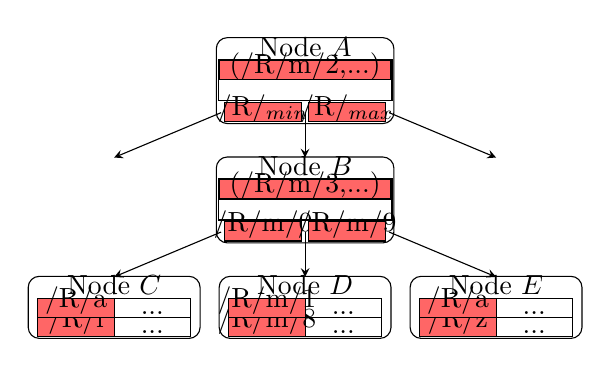
\begin{tikzpicture}
    \node[anchor=south, rectangle, rounded corners, minimum width=.18\textwidth, minimum height=.065\textwidth, draw=black] at (0, 0) {};
    \node[anchor=south] at (0, .036\textwidth) {Node $D$};
    \node[anchor=south, rectangle, minimum width=.08\textwidth, minimum height=.02\textwidth, draw=black, fill={red!60}] at (-.04\textwidth, .002\textwidth) {};
    \node[anchor=south] at (-.04\textwidth, -0.005\textwidth) {/R/m/8};
    \node[anchor=south, rectangle, minimum width=.08\textwidth, minimum height=.02\textwidth, draw=black] at (.04\textwidth, .002\textwidth) {};
    \node[anchor=south] at (.04\textwidth, -0.005\textwidth) {...};
    \node[anchor=south, rectangle, minimum width=.08\textwidth, minimum height=.02\textwidth, draw=black, fill={red!60}] at (-.04\textwidth, .022\textwidth) {};
    \node[anchor=south] at (-.04\textwidth, .015\textwidth) {/R/m/1};
    \node[anchor=south, rectangle, minimum width=.08\textwidth, minimum height=.02\textwidth, draw=black] at (.04\textwidth, .022\textwidth) {};
    \node[anchor=south] at (.04\textwidth, .015\textwidth) {...};

    \node[anchor=south, rectangle, rounded corners, minimum width=.18\textwidth, minimum height=.065\textwidth, draw=black] at (-.2\textwidth, 0) {};
    \node[anchor=south] at (-.2\textwidth, .036\textwidth) {Node $C$};
    \node[anchor=south, rectangle, minimum width=.08\textwidth, minimum height=.02\textwidth, draw=black, fill={red!60}] at (-.24\textwidth, .002\textwidth) {};
    \node[anchor=south] at (-.24\textwidth, -0.005\textwidth) {/R/l};
    \node[anchor=south, rectangle, minimum width=.08\textwidth, minimum height=.02\textwidth, draw=black] at (-.16\textwidth, .002\textwidth) {};
    \node[anchor=south] at (-.16\textwidth, -0.005\textwidth) {...};
    \node[anchor=south, rectangle, minimum width=.08\textwidth, minimum height=.02\textwidth, draw=black, fill={red!60}] at (-.24\textwidth, .022\textwidth) {};
    \node[anchor=south] at (-.24\textwidth, .015\textwidth) {/R/a};
    \node[anchor=south, rectangle, minimum width=.08\textwidth, minimum height=.02\textwidth, draw=black] at (-.16\textwidth, .022\textwidth) {};
    \node[anchor=south] at (-.16\textwidth, .015\textwidth) {...};

    \node[anchor=south, rectangle, rounded corners, minimum width=.18\textwidth, minimum height=.065\textwidth, draw=black] at (.2\textwidth, 0) {};
    \node[anchor=south] at (.2\textwidth, .036\textwidth) {Node $E$};
    \node[anchor=south, rectangle, minimum width=.08\textwidth, minimum height=.02\textwidth, draw=black, fill={red!60}] at (.16\textwidth, .002\textwidth) {};
    \node[anchor=south] at (.16\textwidth, -0.005\textwidth) {/R/z};
    \node[anchor=south, rectangle, minimum width=.08\textwidth, minimum height=.02\textwidth, draw=black] at (.24\textwidth, .002\textwidth) {};
    \node[anchor=south] at (.24\textwidth, -0.005\textwidth) {...};
    \node[anchor=south, rectangle, minimum width=.08\textwidth, minimum height=.02\textwidth, draw=black, fill={red!60}] at (.16\textwidth, .022\textwidth) {};
    \node[anchor=south] at (.16\textwidth, .015\textwidth) {/R/a};
    \node[anchor=south, rectangle, minimum width=.08\textwidth, minimum height=.02\textwidth, draw=black] at (.24\textwidth, .022\textwidth) {};
    \node[anchor=south] at (.24\textwidth, .015\textwidth) {...};

    \node[anchor=south, rectangle, rounded corners, minimum width=.186\textwidth, minimum height=.09\textwidth, draw=black] at (0, .1\textwidth) {};
    \node[anchor=south] at (0, .161\textwidth) {Node $B$};
    \node[anchor=south, rectangle, minimum width=.08\textwidth, minimum height=.02\textwidth, draw=black, fill={red!60}] at (-.044\textwidth, .102\textwidth) {};
    \node[anchor=south] at (-.044\textwidth, .095\textwidth) {/R/m/0};
    \node[anchor=south, rectangle, minimum width=.08\textwidth, minimum height=.02\textwidth, draw=black, fill={red!60}] at (.044\textwidth, .102\textwidth) {};
    \node[anchor=south] at (.044\textwidth, .095\textwidth) {/R/m/9};
    \node[anchor=south, rectangle, minimum width=.182\textwidth, minimum height=.043\textwidth, draw=black] at (0, .124\textwidth) {};
    \node[anchor=south, rectangle, minimum width=.18\textwidth, minimum height=.02\textwidth, draw=black, fill={red!60}] at (0, .146\textwidth) {};
    \node[anchor=south] at  (0, .136\textwidth) {\putm(/R/m/3,...)};

    \node[anchor=south, rectangle, rounded corners, minimum width=.186\textwidth, minimum height=.09\textwidth, draw=black] at (0, .225\textwidth) {};
    \node[anchor=south] at (0, .286\textwidth) {Node $A$};
    \node[anchor=south, rectangle, minimum width=.08\textwidth, minimum height=.02\textwidth, draw=black, fill={red!60}] at (-.044\textwidth, .227\textwidth) {};
    \node[anchor=south] at (-.044\textwidth, .217\textwidth) {/R/$_{min}$};
    \node[anchor=south, rectangle, minimum width=.08\textwidth, minimum height=.02\textwidth, draw=black, fill={red!60}] at (.044\textwidth, .227\textwidth) {};
    \node[anchor=south] at (.044\textwidth, .217\textwidth) {/R/$_{max}$};
    \node[anchor=south, rectangle, minimum width=.182\textwidth, minimum height=.043\textwidth, draw=black] at (0, .249\textwidth) {};
    \node[anchor=south, rectangle, minimum width=.18\textwidth, minimum height=.02\textwidth, draw=black, fill={red!60}] at (0, .271\textwidth) {};
    \node[anchor=south] at  (0, .261\textwidth) {\putm(/R/m/2,...)};

    \draw[->, >=stealth] (-.088\textwidth, .112\textwidth) -- (-.2\textwidth, .065\textwidth);
    \draw[->, >=stealth] (0, .112\textwidth) -- (0, .065\textwidth);
    \draw[->, >=stealth] (.088\textwidth, .112\textwidth) -- (.2\textwidth, .065\textwidth);
    \draw[->, >=stealth] (-.088\textwidth, .237\textwidth) -- (-.2\textwidth, .19\textwidth);
    \draw[->, >=stealth] (0, .237\textwidth) -- (0, .19\textwidth);
    \draw[->, >=stealth] (.088\textwidth, .237\textwidth) -- (.2\textwidth, .19\textwidth);
\end{tikzpicture}

        \caption{\label{subfig:lift-0} A \bet without key lifting.}
    \end{subfigure}
    \begin{subfigure}{\textwidth}
        \centering
        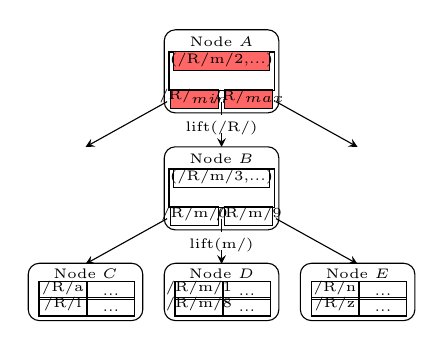
\begin{tikzpicture}[xscale=0.95, yscale=0.95]
            \node[anchor=south, rectangle, rounded corners, minimum height=.06\textwidth, minimum width=.12\textwidth, draw=black] at (0, 0) {};
            \node[anchor=south, font=\tiny] at (0, .036\textwidth) {Node $D$};
            \node[anchor=south, rectangle, minimum height=.015\textwidth, minimum width=.05\textwidth, draw=black] at (-.025\textwidth, .005\textwidth) {};
            \node[anchor=south, font=\tiny] at (-.025\textwidth, 0) {\st{/R/m/}8};
            \node[anchor=south, rectangle, minimum height=.015\textwidth, minimum width=.05\textwidth, draw=black] at (.028\textwidth, .005\textwidth) {};
            \node[anchor=south, font=\tiny] at (.028\textwidth, 0) {...};
            \node[anchor=south, rectangle, minimum height=.015\textwidth, minimum width=.05\textwidth, draw=black] at (-.025\textwidth, .023\textwidth) {};
            \node[anchor=south, font=\tiny] at (-.025\textwidth, .018\textwidth) {\st{/R/m/}1};
            \node[anchor=south, rectangle, minimum height=.015\textwidth, minimum width=.05\textwidth, draw=black] at (.028\textwidth, .023\textwidth) {};
            \node[anchor=south, font=\tiny] at (.028\textwidth, .018\textwidth) {...};

            \node[anchor=south, rectangle, rounded corners, minimum height=.06\textwidth, minimum width=.12\textwidth, draw=black] at (.15\textwidth, 0) {};
            \node[anchor=south, font=\tiny] at (.15\textwidth, .036\textwidth) {Node $E$};
            \node[anchor=south, rectangle, minimum height=.015\textwidth, minimum width=.05\textwidth, draw=black] at (.125\textwidth, .005\textwidth) {};
            \node[anchor=south, font=\tiny] at (.125\textwidth, 0) {\st{/R/}z};
            \node[anchor=south, rectangle, minimum height=.015\textwidth, minimum width=.05\textwidth, draw=black] at (.178\textwidth, .005\textwidth) {};
            \node[anchor=south, font=\tiny] at (.178\textwidth, 0) {...};
            \node[anchor=south, rectangle, minimum height=.015\textwidth, minimum width=.05\textwidth, draw=black] at (.125\textwidth, .023\textwidth) {};
            \node[anchor=south, font=\tiny] at (.125\textwidth, .018\textwidth) {\st{/R/}n};
            \node[anchor=south, rectangle, minimum height=.015\textwidth, minimum width=.05\textwidth, draw=black] at (.178\textwidth, .023\textwidth) {};
            \node[anchor=south, font=\tiny] at (.178\textwidth, .018\textwidth) {...};

            \node[anchor=south, rectangle, rounded corners, minimum height=.06\textwidth, minimum width=.12\textwidth, draw=black] at (-.15\textwidth, 0) {};
            \node[anchor=south, font=\tiny] at (-.15\textwidth, .036\textwidth) {Node $C$};
            \node[anchor=south, rectangle, minimum height=.015\textwidth, minimum width=.05\textwidth, draw=black] at (-.175\textwidth, .005\textwidth) {};
            \node[anchor=south, font=\tiny] at (-.175\textwidth, 0) {\st{/R/}l};
            \node[anchor=south, rectangle, minimum height=.015\textwidth, minimum width=.05\textwidth, draw=black] at (-.122\textwidth, .005\textwidth) {};
            \node[anchor=south, font=\tiny] at (-.122\textwidth, 0) {...};
            \node[anchor=south, rectangle, minimum height=.015\textwidth, minimum width=.05\textwidth, draw=black] at (-.175\textwidth, .023\textwidth) {};
            \node[anchor=south, font=\tiny] at (-.175\textwidth, .018\textwidth) {\st{/R/}a};
            \node[anchor=south, rectangle, minimum height=.015\textwidth, minimum width=.05\textwidth, draw=black] at (-.122\textwidth, .023\textwidth) {};
            \node[anchor=south, font=\tiny] at (-.122\textwidth, .018\textwidth) {...};

            \node[anchor=south, rectangle, rounded corners, minimum height=.087\textwidth, minimum width=.12\textwidth, draw=black] at (0, .1\textwidth) {};
            \node[anchor=south, font=\tiny] at (0, .163\textwidth) {Node $B$};
            \node[anchor=south, rectangle, minimum height=.015\textwidth, minimum width=.05\textwidth, draw=black] at (-.03\textwidth, .105\textwidth) {};
            \node[anchor=south, font=\tiny] at (-.03\textwidth, .1\textwidth) {\st{/R/}m/0};
            \node[anchor=south, rectangle, minimum height=.015\textwidth, minimum width=.05\textwidth, draw=black] at (.03\textwidth, .105\textwidth) {};
            \node[anchor=south, font=\tiny] at (.03\textwidth, .1\textwidth) {\st{/R/}m/9};
            \node[anchor=south, rectangle, minimum height=.04\textwidth, minimum width=.11\textwidth, draw=black] at (0, .125\textwidth) {};
            \node[anchor=south, rectangle, minimum height=.015\textwidth, minimum width=.1\textwidth, draw=black] at (0, .147\textwidth) {};
            \node[anchor=south, font=\tiny] at  (0, .141\textwidth) {\putm(\st{/R/}m/3,...)};

            \node[anchor=south, rectangle, rounded corners, minimum height=.087\textwidth, minimum width=.12\textwidth, draw=black] at (0, .229\textwidth) {};
            \node[anchor=south, font=\tiny] at (0, .292\textwidth) {Node $A$};
            \node[anchor=south, rectangle, minimum height=.015\textwidth, minimum width=.05\textwidth, draw=black, fill={red!60}] at (-.03\textwidth, .234\textwidth) {};
            \node[anchor=south, font=\tiny] at (-.03\textwidth, .229\textwidth) {/R/$_{min}$};
            \node[anchor=south, rectangle, minimum height=.015\textwidth, minimum width=.05\textwidth, draw=black, fill={red!60}] at (.03\textwidth, .234\textwidth) {};
            \node[anchor=south, font=\tiny] at (.03\textwidth, .229\textwidth) {/R/$_{max}$};
            \node[anchor=south, rectangle, minimum height=.04\textwidth, minimum width=.11\textwidth, draw=black] at (0, .254\textwidth) {};
            \node[anchor=south, rectangle, minimum height=.015\textwidth, minimum width=.1\textwidth, draw=black, fill={red!60}] at (0, .276\textwidth) {};
            \node[anchor=south, font=\tiny] at  (0, .27\textwidth) {\putm(/R/m/2,...)};

            \draw[->, >=stealth] (0, .113\textwidth) -- (0, .063\textwidth);
            \draw[->, >=stealth] (.06\textwidth, .113\textwidth) -- (.15\textwidth, .063\textwidth);
            \draw[->, >=stealth] (-.06\textwidth, .113\textwidth) -- (-.15\textwidth, .063\textwidth);
            \draw[->, >=stealth] (0, .242\textwidth) -- (0, .192\textwidth);
            \draw[->, >=stealth] (.06\textwidth, .242\textwidth) -- (.15\textwidth, .192\textwidth);
            \draw[->, >=stealth] (-.06\textwidth, .242\textwidth) -- (-.15\textwidth, .192\textwidth);

            \node[anchor=north,rectangle, minimum height=.015\textwidth, minimum width=.05\textwidth, fill={white}] at (0, .228\textwidth) {};
            \node[anchor=north, font=\tiny] at (0, .231\textwidth) {lift(/R/)};
            \node[anchor=north,rectangle, minimum height=.015\textwidth, minimum width=.05\textwidth, fill={white}] at (0, .099\textwidth) {};
            \node[anchor=north, font=\tiny] at (0, .102\textwidth) {lift(m/)};
        \end{tikzpicture}
        \caption{\label{subfig:lift-1} The lifted \bet that stores the same keys
            in each node. Lifted prefixes are marked as strike-through in keys.}
    \end{subfigure}
    \begin{subfigure}{\textwidth}
        \centering
        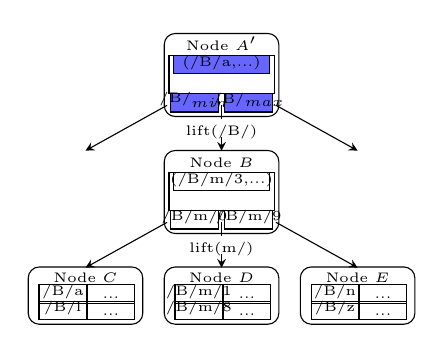
\begin{tikzpicture}[xscale=0.95, yscale=0.95]
            \node[anchor=south, rectangle, rounded corners, minimum height=.06\textwidth, minimum width=.12\textwidth, draw=black] at (0, 0) {};
            \node[anchor=south, font=\tiny] at (0, .036\textwidth) {Node $D$};
            \node[anchor=south, rectangle, minimum height=.015\textwidth, minimum width=.05\textwidth, draw=black] at (-.025\textwidth, .005\textwidth) {};
            \node[anchor=south, font=\tiny] at (-.025\textwidth, 0) {\st{/B/m/}8};
            \node[anchor=south, rectangle, minimum height=.015\textwidth, minimum width=.05\textwidth, draw=black] at (.028\textwidth, .005\textwidth) {};
            \node[anchor=south, font=\tiny] at (.028\textwidth, 0) {...};
            \node[anchor=south, rectangle, minimum height=.015\textwidth, minimum width=.05\textwidth, draw=black] at (-.025\textwidth, .023\textwidth) {};
            \node[anchor=south, font=\tiny] at (-.025\textwidth, .018\textwidth) {\st{/B/m/}1};
            \node[anchor=south, rectangle, minimum height=.015\textwidth, minimum width=.05\textwidth, draw=black] at (.028\textwidth, .023\textwidth) {};
            \node[anchor=south, font=\tiny] at (.028\textwidth, .018\textwidth) {...};

            \node[anchor=south, rectangle, rounded corners, minimum height=.06\textwidth, minimum width=.12\textwidth, draw=black] at (.15\textwidth, 0) {};
            \node[anchor=south, font=\tiny] at (.15\textwidth, .036\textwidth) {Node $E$};
            \node[anchor=south, rectangle, minimum height=.015\textwidth, minimum width=.05\textwidth, draw=black] at (.125\textwidth, .005\textwidth) {};
            \node[anchor=south, font=\tiny] at (.125\textwidth, 0) {\st{/B/}z};
            \node[anchor=south, rectangle, minimum height=.015\textwidth, minimum width=.05\textwidth, draw=black] at (.178\textwidth, .005\textwidth) {};
            \node[anchor=south, font=\tiny] at (.178\textwidth, 0) {...};
            \node[anchor=south, rectangle, minimum height=.015\textwidth, minimum width=.05\textwidth, draw=black] at (.125\textwidth, .023\textwidth) {};
            \node[anchor=south, font=\tiny] at (.125\textwidth, .018\textwidth) {\st{/B/}n};
            \node[anchor=south, rectangle, minimum height=.015\textwidth, minimum width=.05\textwidth, draw=black] at (.178\textwidth, .023\textwidth) {};
            \node[anchor=south, font=\tiny] at (.178\textwidth, .018\textwidth) {...};

            \node[anchor=south, rectangle, rounded corners, minimum height=.06\textwidth, minimum width=.12\textwidth, draw=black] at (-.15\textwidth, 0) {};
            \node[anchor=south, font=\tiny] at (-.15\textwidth, .036\textwidth) {Node $C$};
            \node[anchor=south, rectangle, minimum height=.015\textwidth, minimum width=.05\textwidth, draw=black] at (-.175\textwidth, .005\textwidth) {};
            \node[anchor=south, font=\tiny] at (-.175\textwidth, 0) {\st{/B/}l};
            \node[anchor=south, rectangle, minimum height=.015\textwidth, minimum width=.05\textwidth, draw=black] at (-.122\textwidth, .005\textwidth) {};
            \node[anchor=south, font=\tiny] at (-.122\textwidth, 0) {...};
            \node[anchor=south, rectangle, minimum height=.015\textwidth, minimum width=.05\textwidth, draw=black] at (-.175\textwidth, .023\textwidth) {};
            \node[anchor=south, font=\tiny] at (-.175\textwidth, .018\textwidth) {\st{/B/}a};
            \node[anchor=south, rectangle, minimum height=.015\textwidth, minimum width=.05\textwidth, draw=black] at (-.122\textwidth, .023\textwidth) {};
            \node[anchor=south, font=\tiny] at (-.122\textwidth, .018\textwidth) {...};

            \node[anchor=south, rectangle, rounded corners, minimum height=.087\textwidth, minimum width=.12\textwidth, draw=black] at (0, .1\textwidth) {};
            \node[anchor=south, font=\tiny] at (0, .163\textwidth) {Node $B$};
            \node[anchor=south, rectangle, minimum height=.015\textwidth, minimum width=.05\textwidth, draw=black] at (-.03\textwidth, .105\textwidth) {};
            \node[anchor=south, font=\tiny] at (-.03\textwidth, .1\textwidth) {\st{/B/}m/0};
            \node[anchor=south, rectangle, minimum height=.015\textwidth, minimum width=.05\textwidth, draw=black] at (.03\textwidth, .105\textwidth) {};
            \node[anchor=south, font=\tiny] at (.03\textwidth, .1\textwidth) {\st{/B/}m/9};
            \node[anchor=south, rectangle, minimum height=.04\textwidth, minimum width=.11\textwidth, draw=black] at (0, .125\textwidth) {};
            \node[anchor=south, rectangle, minimum height=.015\textwidth, minimum width=.1\textwidth, draw=black] at (0, .147\textwidth) {};
            \node[anchor=south, font=\tiny] at  (0, .141\textwidth) {\putm(\st{/B/}m/3,...)};

            \node[anchor=south, rectangle, rounded corners, minimum height=.087\textwidth, minimum width=.12\textwidth, draw=black] at (0, .229\textwidth) {};
            \node[anchor=south, font=\tiny] at (0, .292\textwidth) {Node $A'$};
            \node[anchor=south, rectangle, minimum height=.015\textwidth, minimum width=.05\textwidth, draw=black, fill={blue!60}] at (-.03\textwidth, .234\textwidth) {};
            \node[anchor=south, font=\tiny] at (-.03\textwidth, .229\textwidth) {/B/$_{min}$};
            \node[anchor=south, rectangle, minimum height=.015\textwidth, minimum width=.05\textwidth, draw=black, fill={blue!60}] at (.03\textwidth, .234\textwidth) {};
            \node[anchor=south, font=\tiny] at (.03\textwidth, .229\textwidth) {/B/$_{max}$};
            \node[anchor=south, rectangle, minimum height=.04\textwidth, minimum width=.11\textwidth, draw=black] at (0, .254\textwidth) {};
            \node[anchor=south, rectangle, minimum height=.015\textwidth, minimum width=.1\textwidth, draw=black, fill={blue!60}] at (0, .276\textwidth) {};
            \node[anchor=south, font=\tiny] at  (0, .27\textwidth) {\putm(/B/a,...)};

            \draw[->, >=stealth] (0, .113\textwidth) -- (0, .063\textwidth);
            \draw[->, >=stealth] (.06\textwidth, .113\textwidth) -- (.15\textwidth, .063\textwidth);
            \draw[->, >=stealth] (-.06\textwidth, .113\textwidth) -- (-.15\textwidth, .063\textwidth);
            \draw[->, >=stealth] (0, .242\textwidth) -- (0, .192\textwidth);
            \draw[->, >=stealth] (.06\textwidth, .242\textwidth) -- (.15\textwidth, .192\textwidth);
            \draw[->, >=stealth] (-.06\textwidth, .242\textwidth) -- (-.15\textwidth, .192\textwidth);

            \node[anchor=north,rectangle, minimum height=.015\textwidth, minimum width=.05\textwidth, fill={white}] at (0, .228\textwidth) {};
            \node[anchor=north, font=\tiny] at (0, .231\textwidth) {lift(/B/)};
            \node[anchor=north,rectangle, minimum height=.015\textwidth, minimum width=.05\textwidth, fill={white}] at (0, .099\textwidth) {};
            \node[anchor=north, font=\tiny] at (0, .102\textwidth) {lift(m/)};
        \end{tikzpicture}
        \caption{\label{subfig:lift-2} When the subtree rooted at Node $B$ is
            bounded by two different pivots, all keys in the subtree change
            their prefixes.}
    \end{subfigure}
    \caption[An key lifting example]{\label{fig:lift}
        Key lifting lifts prefixes from the subtree. Keys in the same subtree
        are viewed with different prefixes when the pivots in its parent
        change.}
\end{figure}

After tree surgery, one can move the isolated subtree to another location in
the \bet.
However, the keys in the subtree will not be coherent with the new location in
the tree.
Thus, as a part of the range-rename operation, the prefixes of keys in this
subtree need to be updated.
A naive approach will traverse the subtree and update all keys.
However, this process costs a lot of I/Os, rewriting every node in the source
subtree.
The particularly concerning case is when the subtree is very large.

Key lifting eliminates the need to update prefixes of keys in the subtree by
transforming \bets into lifted \bets.
The idea of key lifting comes from the observation that with lexicographic key
order, all keys bounded in the key range of two pivots must have the same prefix
that is the \textbf{LCP} (Longest Common Prefix) of the pivots.
Therefore, this LCP is redundant information in the subtree of the two pivots
and can be removed from the subtree.
In particular, the subtree generated by tree surgery is bounded by two pivots,
$p_{min}$ and $p_{max}$ and with lexicographic key order, all keys in the
subtree must have prefix $p$.

In lifted \bets, a parent-to-child pointer lifts the LCP of the two pivots from
the subtree rooted at the child.
Child nodes only store differing key suffixes.
This approach encodes the complete key in the path taken to reach a given node
and one can then modify the prefix for a lifted subtree by only modifying the
parent node, eliminating the need to change key and pivot prefixes in all nodes
of a subtree.

Figure~\ref{fig:lift} shows an example of key lifting.
Figure~\ref{subfig:lift-0} and Figure~\ref{subfig:lift-1} show the same \bet
with and without key lifting, respectively.
In Figure~\ref{subfig:lift-1}, the subtree rooted at Node $B$ is
bounded by two pivots, ``/R/$_{min}$'' and ``/R/$_{max}$'', in Node $A$.
Therefore, all keys in the subtree must have prefix ``/R/'' and key lifting
removes this prefix from the subtree
(we show the lifted prefix on the parent-to-child pointer and mark the lifted
prefix as strike-through in the subtree).
Because keys in Node $B$ don't have prefix ``/R/'' physically in the node,
we show transparent keys (``/R/'' keys are red in previous examples) in the node.
Likewise, Node $D$ is bounded by ``m/a'' and ``m/z'' in Node $B$
(note ``/R/'' is already lifted from the sutbree rooted at Node $B$),
so key lifting removes prefix ``m/'' from Node $D$.
In Figure~\ref{subfig:lift-2}, the same subtree, which contains exactly the
same key/value pairs, is moved to a different location, bounded by two new
pivots, ``/B/$_{min}$'' and ``/B/$_{max}$'', in Node $A'$.
Because the prefix lifted through the parent-to-child pointer in Node $A'$
becomes ``/B/'', all keys in the subtree have prefix ``/B/'' instead.
For examples in the rest of the dissertation, we will not show lifted prefixes
in keys.

A query on a lifted \bet needs to track lifted prefixes during the
root-to-leaf traversal and reconstruct the full key by concatenating these
prefixes and the suffix in the leaf.
For example, consider a query for key ``/R/m/1'' in Figure~\ref{subfig:lift-1}.
When following the parent-to-child pointer from Node $A$ to Node $B$,
the query notices the lifted prefix ``/R/''.
Therefore, the query searches for key ``m/1'' in Node $B$ and follows the
parent-to-child pointer to Node $D$.
Again, the query removes the lifted prefix, ``m/'', from the search key.
After fetching the key/value pair of key ``1'' in Node $D$, the query prepends
prefixes lifted long the root-to-leaf path and recovers the full key ``/R/m/1''.
Note the recovering process is not necessary for point queries because they know
their keys beforehand, but range queries must reconstruct the resulting keys.

Also, a lifted \bet must remove the lifted prefix from a message before flushing
the message from parent to child.
For example, in Figure~\ref{subfig:lift-1}, when flushing the message
\putm(``/R/m/2'',...) from Node $A$ to Node $B$, the lifted \bet remove the
prefix ``/R/'' from the message and injects a message \putm(``m/2'',...) into
the buffer of Node $B$.

A node split in a lifted \bet adds a pivot to the parent, which may change
the lifted prefix associated with the parent-to-child pointer, so it may need to
update keys in the resulting children.
Similarly, a node merge needs to re-lift keys in the resulting node.

However, the extra work described above for \bet operations can be resolved in
memory.
Therefore, key lifting doesn't incur additional I/Os for other \bet operations.

Compared to zoning, in which the file system removes certain prefixes from keys,
key lifting is completely transparent to \betrfs.
\betrfs still stores key/value pairs with full-path keys,
just with a slightly different data structure.

\subsection{The range-rename operation on lifted \bets}
\label{sec:rr:op:rr}

\begin{figure}
    \begin{subfigure}{\textwidth}
        \centering
        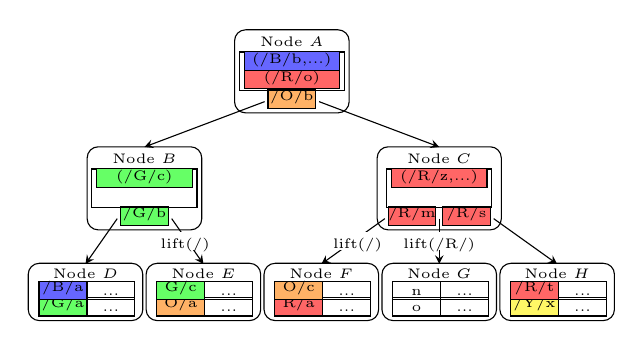
\begin{tikzpicture}[xscale=0.95, yscale=0.95]
            \node[anchor=south, rectangle, rounded corners, minimum height=.06\textwidth, minimum width=.12\textwidth, draw=black] at (0, 0) {};
            \node[anchor=south, font=\tiny] at (0, .036\textwidth) {Node $F$};
            \node[anchor=south, rectangle, minimum height=.015\textwidth, minimum width=.05\textwidth, draw=black, fill={red!60}] at (-.025\textwidth, .005\textwidth) {};
            \node[anchor=south, font=\tiny] at (-.025\textwidth, 0) {R/a};
            \node[anchor=south, rectangle, minimum height=.015\textwidth, minimum width=.05\textwidth, draw=black] at (.028\textwidth, .005\textwidth) {};
            \node[anchor=south, font=\tiny] at (.028\textwidth, 0) {...};
            \node[anchor=south, rectangle, minimum height=.015\textwidth, minimum width=.05\textwidth, draw=black, fill={orange!60}] at (-.025\textwidth, .023\textwidth) {};
            \node[anchor=south, font=\tiny] at (-.025\textwidth, .018\textwidth) {O/c};
            \node[anchor=south, rectangle, minimum height=.015\textwidth, minimum width=.05\textwidth, draw=black] at (.028\textwidth, .023\textwidth) {};
            \node[anchor=south, font=\tiny] at (.028\textwidth, .018\textwidth) {...};

            \node[anchor=south, rectangle, rounded corners, minimum height=.06\textwidth, minimum width=.12\textwidth, draw=black] at (.13\textwidth, 0) {};
            \node[anchor=south, font=\tiny] at (.13\textwidth, .036\textwidth) {Node $G$};
            \node[anchor=south, rectangle, minimum height=.015\textwidth, minimum width=.05\textwidth, draw=black] at (.105\textwidth, .005\textwidth) {};
            \node[anchor=south, font=\tiny] at (.105\textwidth, 0) {o};
            \node[anchor=south, rectangle, minimum height=.015\textwidth, minimum width=.05\textwidth, draw=black] at (.158\textwidth, .005\textwidth) {};
            \node[anchor=south, font=\tiny] at (.158\textwidth, 0) {...};
            \node[anchor=south, rectangle, minimum height=.015\textwidth, minimum width=.05\textwidth, draw=black] at (.105\textwidth, .023\textwidth) {};
            \node[anchor=south, font=\tiny] at (.105\textwidth, .018\textwidth) {n};
            \node[anchor=south, rectangle, minimum height=.015\textwidth, minimum width=.05\textwidth, draw=black] at (.158\textwidth, .023\textwidth) {};
            \node[anchor=south, font=\tiny] at (.158\textwidth, .018\textwidth) {...};

            \node[anchor=south, rectangle, rounded corners, minimum height=.06\textwidth, minimum width=.12\textwidth, draw=black] at (.26\textwidth, 0) {};
            \node[anchor=south, font=\tiny] at (.26\textwidth, .036\textwidth) {Node $H$};
            \node[anchor=south, rectangle, minimum height=.015\textwidth, minimum width=.05\textwidth, draw=black, fill={yellow!60}] at (.235\textwidth, .005\textwidth) {};
            \node[anchor=south, font=\tiny] at (.235\textwidth, 0) {/Y/x};
            \node[anchor=south, rectangle, minimum height=.015\textwidth, minimum width=.05\textwidth, draw=black] at (.288\textwidth, .005\textwidth) {};
            \node[anchor=south, font=\tiny] at (.288\textwidth, 0) {...};
            \node[anchor=south, rectangle, minimum height=.015\textwidth, minimum width=.05\textwidth, draw=black, fill={red!60}] at (.235\textwidth, .023\textwidth) {};
            \node[anchor=south, font=\tiny] at (.235\textwidth, .018\textwidth) {/R/t};
            \node[anchor=south, rectangle, minimum height=.015\textwidth, minimum width=.05\textwidth, draw=black] at (.288\textwidth, .023\textwidth) {};
            \node[anchor=south, font=\tiny] at (.288\textwidth, .018\textwidth) {...};

            \node[anchor=south, rectangle, rounded corners, minimum height=.06\textwidth, minimum width=.12\textwidth, draw=black] at (-.13\textwidth, 0) {};
            \node[anchor=south, font=\tiny] at (-.13\textwidth, .036\textwidth) {Node $E$};
            \node[anchor=south, rectangle, minimum height=.015\textwidth, minimum width=.05\textwidth, draw=black, fill={orange!60}] at (-.155\textwidth, .005\textwidth) {};
            \node[anchor=south, font=\tiny] at (-.155\textwidth, 0) {O/a};
            \node[anchor=south, rectangle, minimum height=.015\textwidth, minimum width=.05\textwidth, draw=black] at (-.102\textwidth, .005\textwidth) {};
            \node[anchor=south, font=\tiny] at (-.102\textwidth, 0) {...};
            \node[anchor=south, rectangle, minimum height=.015\textwidth, minimum width=.05\textwidth, draw=black, fill={green!60}] at (-.155\textwidth, .023\textwidth) {};
            \node[anchor=south, font=\tiny] at (-.155\textwidth, .018\textwidth) {G/c};
            \node[anchor=south, rectangle, minimum height=.015\textwidth, minimum width=.05\textwidth, draw=black] at (-.102\textwidth, .023\textwidth) {};
            \node[anchor=south, font=\tiny] at (-.102\textwidth, .018\textwidth) {...};

            \node[anchor=south, rectangle, rounded corners, minimum height=.06\textwidth, minimum width=.12\textwidth, draw=black] at (-.26\textwidth, 0) {};
            \node[anchor=south, font=\tiny] at (-.26\textwidth, .036\textwidth) {Node $D$};
            \node[anchor=south, rectangle, minimum height=.015\textwidth, minimum width=.05\textwidth, draw=black, fill={green!60}] at (-.285\textwidth, .005\textwidth) {};
            \node[anchor=south, font=\tiny] at (-.285\textwidth, 0) {/G/a};
            \node[anchor=south, rectangle, minimum height=.015\textwidth, minimum width=.05\textwidth, draw=black] at (-.232\textwidth, .005\textwidth) {};
            \node[anchor=south, font=\tiny] at (-.232\textwidth, 0) {...};
            \node[anchor=south, rectangle, minimum height=.015\textwidth, minimum width=.05\textwidth, draw=black, fill={blue!60}] at (-.285\textwidth, .023\textwidth) {};
            \node[anchor=south, font=\tiny] at (-.285\textwidth, .018\textwidth) {/B/a};
            \node[anchor=south, rectangle, minimum height=.015\textwidth, minimum width=.05\textwidth, draw=black] at (-.232\textwidth, .023\textwidth) {};
            \node[anchor=south, font=\tiny] at (-.232\textwidth, .018\textwidth) {...};

            \node[anchor=south, rectangle, rounded corners, minimum height=.087\textwidth, minimum width=.12\textwidth, draw=black] at (-.195\textwidth, .1\textwidth) {};
            \node[anchor=south, font=\tiny] at (-.195\textwidth, .163\textwidth) {Node $B$};
            \node[anchor=south, rectangle, minimum height=.015\textwidth, minimum width=.05\textwidth, draw=black, fill={green!60}] at (-.195\textwidth, .105\textwidth) {};
            \node[anchor=south, font=\tiny] at (-.195\textwidth, .1\textwidth) {/G/b};
            \node[anchor=south, rectangle, minimum height=.04\textwidth, minimum width=.11\textwidth, draw=black] at (-.195\textwidth, .125\textwidth) {};
            \node[anchor=south, rectangle, minimum height=.015\textwidth, minimum width=.1\textwidth, draw=black, fill={green!60}] at (-.195\textwidth, .147\textwidth) {};
            \node[anchor=south, font=\tiny] at  (-.195\textwidth, .141\textwidth) {\delm(/G/c)};

            \node[anchor=south, rectangle, rounded corners, minimum height=.087\textwidth, minimum width=.13\textwidth, draw=black] at (.13\textwidth, .1\textwidth) {};
            \node[anchor=south, font=\tiny] at (.13\textwidth, .163\textwidth) {Node $C$};
            \node[anchor=south, rectangle, minimum height=.015\textwidth, minimum width=.05\textwidth, draw=black, fill={red!60}] at (.1\textwidth, .105\textwidth) {};
            \node[anchor=south, font=\tiny] at (.1\textwidth, .1\textwidth) {/R/m};
            \node[anchor=south, rectangle, minimum height=.015\textwidth, minimum width=.05\textwidth, draw=black, fill={red!60}] at (.16\textwidth, .105\textwidth) {};
            \node[anchor=south, font=\tiny] at (.16\textwidth, .1\textwidth) {/R/s};
            \node[anchor=south, rectangle, minimum height=.04\textwidth, minimum width=.11\textwidth, draw=black] at (.13\textwidth, .125\textwidth) {};
            \node[anchor=south, rectangle, minimum height=.015\textwidth, minimum width=.1\textwidth, draw=black, fill={red!60}] at (.13\textwidth, .147\textwidth) {};
            \node[anchor=south, font=\tiny] at  (.13\textwidth, .141\textwidth) {\putm(/R/z,...)};

            \node[anchor=south, rectangle, rounded corners, minimum height=.087\textwidth, minimum width=.12\textwidth, draw=black] at (-.0325\textwidth, .229\textwidth) {};
            \node[anchor=south, font=\tiny] at (-.0325\textwidth, .292\textwidth) {Node $A$};
            \node[anchor=south, rectangle, minimum height=.015\textwidth, minimum width=.05\textwidth, draw=black, fill={orange!60}] at (-.0325\textwidth, .234\textwidth) {};
            \node[anchor=south, font=\tiny] at (-.0325\textwidth, .229\textwidth) {/O/b};
            \node[anchor=south, rectangle, minimum height=.04\textwidth, minimum width=.11\textwidth, draw=black] at (-.0325\textwidth, .254\textwidth) {};
            \node[anchor=south, rectangle, minimum height=.015\textwidth, minimum width=.1\textwidth, draw=black, fill={red!60}] at (-.0325\textwidth, .256\textwidth) {};
            \node[anchor=south, font=\tiny] at  (-.0325\textwidth, .25\textwidth) {\delm(/R/o)};
            \node[anchor=south, rectangle, minimum height=.015\textwidth, minimum width=.1\textwidth, draw=black, fill={blue!60}] at (-.0325\textwidth, .276\textwidth) {};
            \node[anchor=south, font=\tiny] at  (-.0325\textwidth, .27\textwidth) {\putm(/B/b,...)};

            \draw[->, >=stealth] (-.225\textwidth, .113\textwidth) -- (-.26\textwidth, .063\textwidth);
            \draw[->, >=stealth] (-.165\textwidth, .113\textwidth) -- (-.13\textwidth, .063\textwidth);
            \draw[->, >=stealth] (.13\textwidth, .113\textwidth) -- (.13\textwidth, .063\textwidth);
            \draw[->, >=stealth] (.19\textwidth, .113\textwidth) -- (.26\textwidth, .063\textwidth);
            \draw[->, >=stealth] (.07\textwidth, .113\textwidth) -- (0, .063\textwidth);
            \draw[->, >=stealth] (-.0625\textwidth, .242\textwidth) -- (-.195\textwidth, .192\textwidth);
            \draw[->, >=stealth] (-.0025\textwidth, .242\textwidth) -- (.13\textwidth, .192\textwidth);

            \node[anchor=north,rectangle, minimum height=.015\textwidth, minimum width=.05\textwidth, fill={white}] at (.13\textwidth, .099\textwidth) {};
            \node[anchor=north, font=\tiny] at (.13\textwidth, .102\textwidth) {lift(/R/)};
            \node[anchor=north,rectangle, minimum height=.015\textwidth, minimum width=.05\textwidth, fill={white}] at (.04\textwidth, .099\textwidth) {};
            \node[anchor=north, font=\tiny] at (.04\textwidth, .102\textwidth) {lift(/)};
            \node[anchor=north,rectangle, minimum height=.015\textwidth, minimum width=.05\textwidth, fill={white}] at (-.15\textwidth, .099\textwidth) {};
            \node[anchor=north, font=\tiny] at (-.15\textwidth, .102\textwidth) {lift(/)};
        \end{tikzpicture}
        \caption{\label{subfig:rr-1} The \bet before the range-rename operation.}
    \end{subfigure}
    \begin{subfigure}{\textwidth}
        \centering
        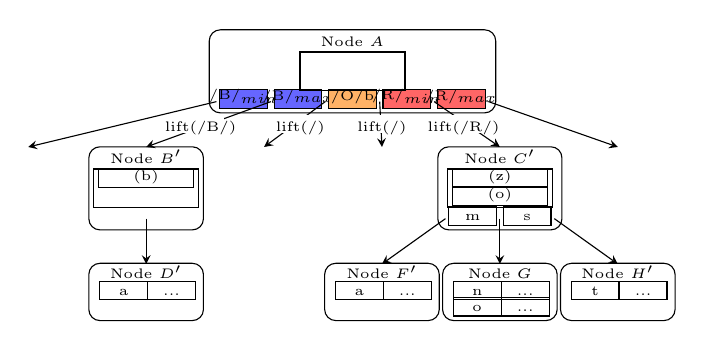
\begin{tikzpicture}[xscale=0.95, yscale=0.95]
            \node[anchor=south, rectangle, rounded corners, minimum height=.06\textwidth, minimum width=.12\textwidth, draw=black] at (0, 0) {};
            \node[anchor=south, font=\tiny] at (0, .036\textwidth) {Node $F'$};
            \node[anchor=south, rectangle, minimum height=.015\textwidth, minimum width=.05\textwidth, draw=black] at (-.025\textwidth, .023\textwidth) {};
            \node[anchor=south, font=\tiny] at (-.025\textwidth, .018\textwidth) {a};
            \node[anchor=south, rectangle, minimum height=.015\textwidth, minimum width=.05\textwidth, draw=black] at (.028\textwidth, .023\textwidth) {};
            \node[anchor=south, font=\tiny] at (.028\textwidth, .018\textwidth) {...};

            \node[anchor=south, rectangle, rounded corners, minimum height=.06\textwidth, minimum width=.12\textwidth, draw=black] at (.13\textwidth, 0) {};
            \node[anchor=south, font=\tiny] at (.13\textwidth, .036\textwidth) {Node $G$};
            \node[anchor=south, rectangle, minimum height=.015\textwidth, minimum width=.05\textwidth, draw=black] at (.105\textwidth, .005\textwidth) {};
            \node[anchor=south, font=\tiny] at (.105\textwidth, 0) {o};
            \node[anchor=south, rectangle, minimum height=.015\textwidth, minimum width=.05\textwidth, draw=black] at (.158\textwidth, .005\textwidth) {};
            \node[anchor=south, font=\tiny] at (.158\textwidth, 0) {...};
            \node[anchor=south, rectangle, minimum height=.015\textwidth, minimum width=.05\textwidth, draw=black] at (.105\textwidth, .023\textwidth) {};
            \node[anchor=south, font=\tiny] at (.105\textwidth, .018\textwidth) {n};
            \node[anchor=south, rectangle, minimum height=.015\textwidth, minimum width=.05\textwidth, draw=black] at (.158\textwidth, .023\textwidth) {};
            \node[anchor=south, font=\tiny] at (.158\textwidth, .018\textwidth) {...};

            \node[anchor=south, rectangle, rounded corners, minimum height=.06\textwidth, minimum width=.12\textwidth, draw=black] at (.26\textwidth, 0) {};
            \node[anchor=south, font=\tiny] at (.26\textwidth, .036\textwidth) {Node $H'$};
            \node[anchor=south, rectangle, minimum height=.015\textwidth, minimum width=.05\textwidth, draw=black] at (.235\textwidth, .023\textwidth) {};
            \node[anchor=south, font=\tiny] at (.235\textwidth, .018\textwidth) {t};
            \node[anchor=south, rectangle, minimum height=.015\textwidth, minimum width=.05\textwidth, draw=black] at (.288\textwidth, .023\textwidth) {};
            \node[anchor=south, font=\tiny] at (.288\textwidth, .018\textwidth) {...};

            \node[anchor=south, rectangle, rounded corners, minimum height=.06\textwidth, minimum width=.12\textwidth, draw=black] at (-.26\textwidth, 0) {};
            \node[anchor=south, font=\tiny] at (-.26\textwidth, .036\textwidth) {Node $D'$};
            \node[anchor=south, rectangle, minimum height=.015\textwidth, minimum width=.05\textwidth, draw=black] at (-.285\textwidth, .023\textwidth) {};
            \node[anchor=south, font=\tiny] at (-.285\textwidth, .018\textwidth) {a};
            \node[anchor=south, rectangle, minimum height=.015\textwidth, minimum width=.05\textwidth, draw=black] at (-.232\textwidth, .023\textwidth) {};
            \node[anchor=south, font=\tiny] at (-.232\textwidth, .018\textwidth) {...};

            \node[anchor=south, rectangle, rounded corners, minimum height=.087\textwidth, minimum width=.12\textwidth, draw=black] at (-.26\textwidth, .1\textwidth) {};
            \node[anchor=south, font=\tiny] at (-.26\textwidth, .163\textwidth) {Node $B'$};
            \node[anchor=south, rectangle, minimum height=.04\textwidth, minimum width=.11\textwidth, draw=black] at (-.26\textwidth, .125\textwidth) {};
            \node[anchor=south, rectangle, minimum height=.015\textwidth, minimum width=.1\textwidth, draw=black] at (-.26\textwidth, .147\textwidth) {};
            \node[anchor=south, font=\tiny] at  (-.26\textwidth, .141\textwidth) {\putm(b)};

            \node[anchor=south, rectangle, rounded corners, minimum height=.087\textwidth, minimum width=.13\textwidth, draw=black] at (.13\textwidth, .1\textwidth) {};
            \node[anchor=south, font=\tiny] at (.13\textwidth, .163\textwidth) {Node $C'$};
            \node[anchor=south, rectangle, minimum height=.015\textwidth, minimum width=.05\textwidth, draw=black] at (.1\textwidth, .105\textwidth) {};
            \node[anchor=south, font=\tiny] at (.1\textwidth, .1\textwidth) {m};
            \node[anchor=south, rectangle, minimum height=.015\textwidth, minimum width=.05\textwidth, draw=black] at (.16\textwidth, .105\textwidth) {};
            \node[anchor=south, font=\tiny] at (.16\textwidth, .1\textwidth) {s};
            \node[anchor=south, rectangle, minimum height=.04\textwidth, minimum width=.11\textwidth, draw=black] at (.13\textwidth, .125\textwidth) {};
            \node[anchor=south, rectangle, minimum height=.015\textwidth, minimum width=.1\textwidth, draw=black] at (.13\textwidth, .147\textwidth) {};
            \node[anchor=south, font=\tiny] at  (.13\textwidth, .141\textwidth) {\putm(z)};
            \node[anchor=south, rectangle, minimum height=.015\textwidth, minimum width=.1\textwidth, draw=black] at (.13\textwidth, .127\textwidth) {};
            \node[anchor=south, font=\tiny] at  (.13\textwidth, .121\textwidth) {\delm(o)};

            \node[anchor=south, rectangle, rounded corners, minimum height=.087\textwidth, minimum width=.3\textwidth, draw=black] at (-.0325\textwidth, .229\textwidth) {};
            \node[anchor=south, font=\tiny] at (-.0325\textwidth, .292\textwidth) {Node $A$};
            \node[anchor=south, rectangle, minimum height=.015\textwidth, minimum width=.05\textwidth, draw=black, fill={blue!60}] at (-.1525\textwidth, .234\textwidth) {};
            \node[anchor=south, font=\tiny] at (-.1525\textwidth, .229\textwidth) {/B/$_{min}$};
            \node[anchor=south, rectangle, minimum height=.015\textwidth, minimum width=.05\textwidth, draw=black, fill={blue!60}] at (-.0925\textwidth, .234\textwidth) {};
            \node[anchor=south, font=\tiny] at (-.0925\textwidth, .229\textwidth) {/B/$_{max}$};
            \node[anchor=south, rectangle, minimum height=.015\textwidth, minimum width=.05\textwidth, draw=black, fill={orange!60}] at (-.0325\textwidth, .234\textwidth) {};
            \node[anchor=south, font=\tiny] at (-.0325\textwidth, .229\textwidth) {/O/b};
            \node[anchor=south, rectangle, minimum height=.015\textwidth, minimum width=.05\textwidth, draw=black, fill={red!60}] at (.0275\textwidth, .234\textwidth) {};
            \node[anchor=south, font=\tiny] at (.0275\textwidth, .229\textwidth) {/R/$_{min}$};
            \node[anchor=south, rectangle, minimum height=.015\textwidth, minimum width=.05\textwidth, draw=black, fill={red!60}] at (.0875\textwidth, .234\textwidth) {};
            \node[anchor=south, font=\tiny] at (.0875\textwidth, .229\textwidth) {/R/$_{max}$};
            \node[anchor=south, rectangle, minimum height=.04\textwidth, minimum width=.11\textwidth, draw=black] at (-.0325\textwidth, .254\textwidth) {};

            \draw[->, >=stealth] (-.26\textwidth, .113\textwidth) -- (-.26\textwidth, .063\textwidth);
            \draw[->, >=stealth] (.13\textwidth, .113\textwidth) -- (.13\textwidth, .063\textwidth);
            \draw[->, >=stealth] (.19\textwidth, .113\textwidth) -- (.26\textwidth, .063\textwidth);
            \draw[->, >=stealth] (.07\textwidth, .113\textwidth) -- (0, .063\textwidth);
            \draw[->, >=stealth] (-.1825\textwidth, .242\textwidth) -- (-.39\textwidth, .192\textwidth);
            \draw[->, >=stealth] (-.1225\textwidth, .242\textwidth) -- (-.26\textwidth, .192\textwidth);
            \draw[->, >=stealth] (-.0625\textwidth, .242\textwidth) -- (-.13\textwidth, .192\textwidth);
            \draw[->, >=stealth] (-.0025\textwidth, .242\textwidth) -- (0, .192\textwidth);
            \draw[->, >=stealth] (.0575\textwidth, .242\textwidth) -- (.13\textwidth, .192\textwidth);
            \draw[->, >=stealth] (.1175\textwidth, .242\textwidth) -- (.26\textwidth, .192\textwidth);

            \node[anchor=north,rectangle, minimum height=.015\textwidth, minimum width=.05\textwidth, fill={white}] at (-.20\textwidth, .228\textwidth) {};
            \node[anchor=north, font=\tiny] at (-.20\textwidth, .231\textwidth) {lift(/B/)};
            \node[anchor=north,rectangle, minimum height=.015\textwidth, minimum width=.05\textwidth, fill={white}] at (-.09\textwidth, .228\textwidth) {};
            \node[anchor=north, font=\tiny] at (-.09\textwidth, .231\textwidth) {lift(/)};
            \node[anchor=north,rectangle, minimum height=.015\textwidth, minimum width=.05\textwidth, fill={white}] at (0, .228\textwidth) {};
            \node[anchor=north, font=\tiny] at (0, .231\textwidth) {lift(/)};
            \node[anchor=north,rectangle, minimum height=.015\textwidth, minimum width=.05\textwidth, fill={white}] at (.09\textwidth, .228\textwidth) {};
            \node[anchor=north, font=\tiny] at (.09\textwidth, .231\textwidth) {lift(/R/)};
        \end{tikzpicture}
        \caption{\label{subfig:rr-2} The range-rename operations performs tree surgery
            to slice out the source and destination subtrees.}
    \end{subfigure}
    \begin{subfigure}{\textwidth}
        \centering
        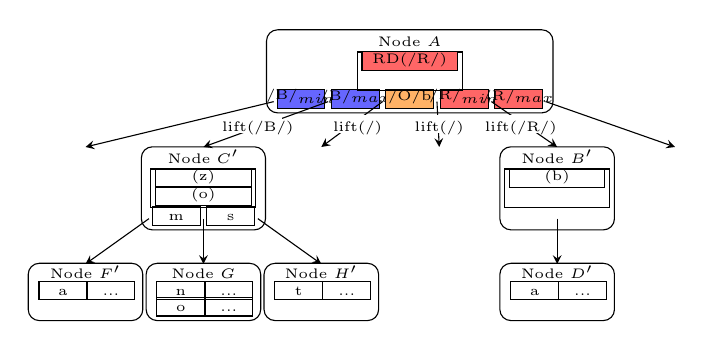
\begin{tikzpicture}[xscale=0.95, yscale=0.95]
            \node[anchor=south, rectangle, rounded corners, minimum height=.06\textwidth, minimum width=.12\textwidth, draw=black] at (-.39\textwidth, 0) {};
            \node[anchor=south, font=\tiny] at (-.39\textwidth, .036\textwidth) {Node $F'$};
            \node[anchor=south, rectangle, minimum height=.015\textwidth, minimum width=.05\textwidth, draw=black] at (-.415\textwidth, .023\textwidth) {};
            \node[anchor=south, font=\tiny] at (-.415\textwidth, .018\textwidth) {a};
            \node[anchor=south, rectangle, minimum height=.015\textwidth, minimum width=.05\textwidth, draw=black] at (-.362\textwidth, .023\textwidth) {};
            \node[anchor=south, font=\tiny] at (-.362\textwidth, .018\textwidth) {...};

            \node[anchor=south, rectangle, rounded corners, minimum height=.06\textwidth, minimum width=.12\textwidth, draw=black] at (-.26\textwidth, 0) {};
            \node[anchor=south, font=\tiny] at (-.26\textwidth, .036\textwidth) {Node $G$};
            \node[anchor=south, rectangle, minimum height=.015\textwidth, minimum width=.05\textwidth, draw=black] at (-.285\textwidth, .005\textwidth) {};
            \node[anchor=south, font=\tiny] at (-.285\textwidth, 0) {o};
            \node[anchor=south, rectangle, minimum height=.015\textwidth, minimum width=.05\textwidth, draw=black] at (-.232\textwidth, .005\textwidth) {};
            \node[anchor=south, font=\tiny] at (-.232\textwidth, 0) {...};
            \node[anchor=south, rectangle, minimum height=.015\textwidth, minimum width=.05\textwidth, draw=black] at (-.285\textwidth, .023\textwidth) {};
            \node[anchor=south, font=\tiny] at (-.285\textwidth, .018\textwidth) {n};
            \node[anchor=south, rectangle, minimum height=.015\textwidth, minimum width=.05\textwidth, draw=black] at (-.232\textwidth, .023\textwidth) {};
            \node[anchor=south, font=\tiny] at (-.232\textwidth, .018\textwidth) {...};

            \node[anchor=south, rectangle, rounded corners, minimum height=.06\textwidth, minimum width=.12\textwidth, draw=black] at (-.13\textwidth, 0) {};
            \node[anchor=south, font=\tiny] at (-.13\textwidth, .036\textwidth) {Node $H'$};
            \node[anchor=south, rectangle, minimum height=.015\textwidth, minimum width=.05\textwidth, draw=black] at (-.155\textwidth, .023\textwidth) {};
            \node[anchor=south, font=\tiny] at (-.155\textwidth, .018\textwidth) {t};
            \node[anchor=south, rectangle, minimum height=.015\textwidth, minimum width=.05\textwidth, draw=black] at (-.102\textwidth, .023\textwidth) {};
            \node[anchor=south, font=\tiny] at (-.102\textwidth, .018\textwidth) {...};

            \node[anchor=south, rectangle, rounded corners, minimum height=.06\textwidth, minimum width=.12\textwidth, draw=black] at (.13\textwidth, 0) {};
            \node[anchor=south, font=\tiny] at (.13\textwidth, .036\textwidth) {Node $D'$};
            \node[anchor=south, rectangle, minimum height=.015\textwidth, minimum width=.05\textwidth, draw=black] at (.105\textwidth, .023\textwidth) {};
            \node[anchor=south, font=\tiny] at (.105\textwidth, .018\textwidth) {a};
            \node[anchor=south, rectangle, minimum height=.015\textwidth, minimum width=.05\textwidth, draw=black] at (.158\textwidth, .023\textwidth) {};
            \node[anchor=south, font=\tiny] at (.158\textwidth, .018\textwidth) {...};

            \node[anchor=south, rectangle, rounded corners, minimum height=.087\textwidth, minimum width=.12\textwidth, draw=black] at (.13\textwidth, .1\textwidth) {};
            \node[anchor=south, font=\tiny] at (.13\textwidth, .163\textwidth) {Node $B'$};
            \node[anchor=south, rectangle, minimum height=.04\textwidth, minimum width=.11\textwidth, draw=black] at (.13\textwidth, .125\textwidth) {};
            \node[anchor=south, rectangle, minimum height=.015\textwidth, minimum width=.1\textwidth, draw=black] at (.13\textwidth, .147\textwidth) {};
            \node[anchor=south, font=\tiny] at  (.13\textwidth, .141\textwidth) {\putm(b)};

            \node[anchor=south, rectangle, rounded corners, minimum height=.087\textwidth, minimum width=.13\textwidth, draw=black] at (-.26\textwidth, .1\textwidth) {};
            \node[anchor=south, font=\tiny] at (-.26\textwidth, .163\textwidth) {Node $C'$};
            \node[anchor=south, rectangle, minimum height=.015\textwidth, minimum width=.05\textwidth, draw=black] at (-.29\textwidth, .105\textwidth) {};
            \node[anchor=south, font=\tiny] at (-.29\textwidth, .1\textwidth) {m};
            \node[anchor=south, rectangle, minimum height=.015\textwidth, minimum width=.05\textwidth, draw=black] at (-.23\textwidth, .105\textwidth) {};
            \node[anchor=south, font=\tiny] at (-.23\textwidth, .1\textwidth) {s};
            \node[anchor=south, rectangle, minimum height=.04\textwidth, minimum width=.11\textwidth, draw=black] at (-.26\textwidth, .125\textwidth) {};
            \node[anchor=south, rectangle, minimum height=.015\textwidth, minimum width=.1\textwidth, draw=black] at (-.26\textwidth, .147\textwidth) {};
            \node[anchor=south, font=\tiny] at  (-.26\textwidth, .141\textwidth) {\putm(z)};
            \node[anchor=south, rectangle, minimum height=.015\textwidth, minimum width=.1\textwidth, draw=black] at (-.26\textwidth, .127\textwidth) {};
            \node[anchor=south, font=\tiny] at  (-.26\textwidth, .121\textwidth) {\delm(o)};

            \node[anchor=south, rectangle, rounded corners, minimum height=.087\textwidth, minimum width=.3\textwidth, draw=black] at (-.0325\textwidth, .229\textwidth) {};
            \node[anchor=south, font=\tiny] at (-.0325\textwidth, .292\textwidth) {Node $A$};
            \node[anchor=south, rectangle, minimum height=.015\textwidth, minimum width=.05\textwidth, draw=black, fill={blue!60}] at (-.1525\textwidth, .234\textwidth) {};
            \node[anchor=south, font=\tiny] at (-.1525\textwidth, .229\textwidth) {/B/$_{min}$};
            \node[anchor=south, rectangle, minimum height=.015\textwidth, minimum width=.05\textwidth, draw=black, fill={blue!60}] at (-.0925\textwidth, .234\textwidth) {};
            \node[anchor=south, font=\tiny] at (-.0925\textwidth, .229\textwidth) {/B/$_{max}$};
            \node[anchor=south, rectangle, minimum height=.015\textwidth, minimum width=.05\textwidth, draw=black, fill={orange!60}] at (-.0325\textwidth, .234\textwidth) {};
            \node[anchor=south, font=\tiny] at (-.0325\textwidth, .229\textwidth) {/O/b};
            \node[anchor=south, rectangle, minimum height=.015\textwidth, minimum width=.05\textwidth, draw=black, fill={red!60}] at (.0275\textwidth, .234\textwidth) {};
            \node[anchor=south, font=\tiny] at (.0275\textwidth, .229\textwidth) {/R/$_{min}$};
            \node[anchor=south, rectangle, minimum height=.015\textwidth, minimum width=.05\textwidth, draw=black, fill={red!60}] at (.0875\textwidth, .234\textwidth) {};
            \node[anchor=south, font=\tiny] at (.0875\textwidth, .229\textwidth) {/R/$_{max}$};
            \node[anchor=south, rectangle, minimum height=.04\textwidth, minimum width=.11\textwidth, draw=black] at (-.0325\textwidth, .254\textwidth) {};
            \node[anchor=south, rectangle, minimum height=.015\textwidth, minimum width=.1\textwidth, draw=black, fill={red!60}] at (-.0325\textwidth, .276\textwidth) {};
            \node[anchor=south, font=\tiny] at  (-.0325\textwidth, .27\textwidth) {RD(/R/)};

            \draw[->, >=stealth] (-.32\textwidth, .113\textwidth) -- (-.39\textwidth, .063\textwidth);
            \draw[->, >=stealth] (-.26\textwidth, .113\textwidth) -- (-.26\textwidth, .063\textwidth);
            \draw[->, >=stealth] (-.20\textwidth, .113\textwidth) -- (-.13\textwidth, .063\textwidth);
            \draw[->, >=stealth] (.13\textwidth, .113\textwidth) -- (.13\textwidth, .063\textwidth);
            \draw[->, >=stealth] (-.1825\textwidth, .242\textwidth) -- (-.39\textwidth, .192\textwidth);
            \draw[->, >=stealth] (-.1225\textwidth, .242\textwidth) -- (-.26\textwidth, .192\textwidth);
            \draw[->, >=stealth] (-.0625\textwidth, .242\textwidth) -- (-.13\textwidth, .192\textwidth);
            \draw[->, >=stealth] (-.0025\textwidth, .242\textwidth) -- (0, .192\textwidth);
            \draw[->, >=stealth] (.0575\textwidth, .242\textwidth) -- (.13\textwidth, .192\textwidth);
            \draw[->, >=stealth] (.1175\textwidth, .242\textwidth) -- (.26\textwidth, .192\textwidth);

            \node[anchor=north,rectangle, minimum height=.015\textwidth, minimum width=.05\textwidth, fill={white}] at (-.20\textwidth, .228\textwidth) {};
            \node[anchor=north, font=\tiny] at (-.20\textwidth, .231\textwidth) {lift(/B/)};
            \node[anchor=north,rectangle, minimum height=.015\textwidth, minimum width=.05\textwidth, fill={white}] at (-.09\textwidth, .228\textwidth) {};
            \node[anchor=north, font=\tiny] at (-.09\textwidth, .231\textwidth) {lift(/)};
            \node[anchor=north,rectangle, minimum height=.015\textwidth, minimum width=.05\textwidth, fill={white}] at (0, .228\textwidth) {};
            \node[anchor=north, font=\tiny] at (0, .231\textwidth) {lift(/)};
            \node[anchor=north,rectangle, minimum height=.015\textwidth, minimum width=.05\textwidth, fill={white}] at (.09\textwidth, .228\textwidth) {};
            \node[anchor=north, font=\tiny] at (.09\textwidth, .231\textwidth) {lift(/R/)};
        \end{tikzpicture}
        \caption{\label{subfig:rr-3} The range-rename operation swaps the subtrees and
            injects a range-delete message for source keys.}
    \end{subfigure}
    \caption[A range-rename example]{\label{fig:rr}
        An example of range-rename(``/R/'', ``/B/'') on the \bet.}
\end{figure}

On a lifted \bet, range-rename(\spre, \dpre) can be done with two steps:

\paragraph{Tree Surgery.}
The range-rename operation first slices out two isolated subtrees in the lifted
\bet simultaneously, one of \spre and the other of \dpre.

\paragraph{Transplant.}
Then, the range-rename operation swaps these two subtrees and injects a
range-delete message for source keys.
Alternatively, one can garbage collect the destination subtree and merge nodes
at the source.
However, garbage collecting the destination subtree requires traversing
the subtree.
Instead, we leverage the existing range-delete message to reclaim the space
of the destination subtree.

Similar to a \btree, a \bet should keep all leaf nodes at the same distance
from the root node.
Otherwise, the \bet becomes unbalanced, breaking the asymptotic I/O cost
analysis.
In order to keep all leaf nodes at the same distance after transplanting,
the range-rename operation requires the source and destination subtrees to be at
the same height.
Therefore, in tree surgery, for the subtree with a lower LCA,
the range-rename operation keeps slicing its ancestors by adding empty nodes
with only one child.

Figure~\ref{fig:rr} shows an example of range-rename(``/R/'', ``/B/'') on the
\bet.
Figure~\ref{subfig:rr-1} shows the lifted \bet before the range-rename
operation.
In Figure~\ref{subfig:rr-2}, the range-rename operation performs tree surgery
to slice out the source subtree, rooted at Node $C'$,
and the destination subtree, rooted at Node $B'$.
Though the destination LCA in Figure~\ref{subfig:rr-1} is Node $D$,
tree surgery still splits Node $B$
to keep the source and destination subtrees at the same height.
Also, prefix ``/R/'' is lifted from the source subtree and prefix ``/B/''
is lifted from the destination subtree.
In the interest of brevity, we omit unrelated nodes generated by tree surgery.
Figure~\ref{subfig:rr-3} shows the lifted \bet after swapping the source and
destination subtrees, with a range-delete message for ``/R/'' keys in Node $A$.
At this point, no key with prefix ``/R/'' exists in the lifted \bet because of
the range-delete message, and all keys with prefix ``/R/'' in
Figure~\ref{subfig:rr-1} now have prefix ``/B/''.

\paragraph{Healing.}
Tree surgery may create undersized \bet nodes,
i.e., non-leaf nodes without enough children,
or leaf nodes without enough key/value pairs.
In a normal node split, the \bet evenly splits a node that is oversized
(a non-leaf node with too many children or
a leaf node with too many key/value pairs),
so the resulting two nodes will not be undersized.
However, tree surgery splits normal nodes with the minimum and maximum
keys of a certain prefix,
which can split the node unevenly.
Moreover, to meet the tree height invariant,
tree surgery may create ``stalks'', non-leaf nodes with only one child,
so that the source and destination subtrees are at the same height.

The range-rename operation handles this situation by
triggering a rebalancing within the tree.
Specifically, if a node has only one child, the slicing process will merge
the node after completing the work of the range-rename operation.
After the transplant completes, there may be a number of \bet nodes in memory at
the fringe around the source and destination that have fewer children than
desired.
The healing process merges these smaller nodes back together,
using the same approach as a typical \bet node merge.

\paragraph{Complexity.}
During tree surgery, at most 4 root-to-leaf paths
(2 for source and 2 for destination) are traversed, dirtying all
nodes along the paths.
These nodes will need to be read, if not in cache, and written back to disk as
part of the checkpointing process.
Therefore, the number of I/Os required in tree surgery is at most proportional
to the height of the \bet, which is logarithmic in the size of the tree.

The healing process only merges nodes that are split during the tree surgery
process.
Therefore, the number of I/Os required in the healing process is also
$O(log_{B}{N}/\varepsilon)$ (tree height).

There is also lifting work along all nodes that are sliced in tree surgery or
merged in healing.
However, the number of such nodes is at most proportional to the height of the
tree.
Thus, the number of nodes that must be lifted during a range-rename is no more
than the nodes that must be sliced during tree surgery, and proportional to
the height of the tree.

In summary, the I/O cost of a range-rename is $O(log_{B}{N}/\varepsilon)$.

\section{Implementation}
\label{sec:rr:impl}

This section discusses implementation details of the range-rename operation.

\subsection{Synchronization}
\label{sec:rr:impl:sync}

The range-rename operation synchronizes with other \bet operations using
the readers-writer locks of \bet nodes
(described in Section~\ref{sec:bg:impl:sync}).
Starting from the root node, the range-rename operation
write-locks \bet nodes hand-over-hand until reaching the LCAs.
To avoid newer messages being flushed to the subtrees rooted at the LCAs,
the write locks of the LCAs and the parents of the LCAs are held until the
range-rename operation completes.
Then, the range-rename operation write-locks all fringe nodes below the LCAs
and releases the write locks after the bottom-up node splits.
After transplanting, the range-rename operation finally releases the write locks
of the LCAs and the parents of the LCAs.

\subsection{Re-lifting a non-leaf node}

Re-lifting a node requires updating prefixes of all keys in the node.
Because \fti has a large node size (4 MiB),
re-lifting a node can cause a large amount of computation.

However, as described in Section~\ref{sec:bg:impl:partition},
\fti stores messages in a non-leaf node in partitions,
each corresponding to a child.
Therefore, we can lift the prefixes of keys in a partition by the
LCP of two pivots bounding it in the non-leaf node.
In other words, keys in the partition are not only lifted by pivots in ancestors
but also the two pivots in the node.
For example, consider a non-leaf node that contains keys in
(``/R/a/1'', ``R/b''),
key lifting lifts prefix ``/R/'' from all keys in the node.
Assume there are two adjacent pivots ``a/2'' and ``a/3'' in the node
(prefix ``/R/'' is lifted).
There is a partition in the node storing all keys in (``/R/a/2'', ``/R/a/3''),
with prefix ``/R/a/'' lifted.

To see how it helps, consider a partition bounded by two pivots in the non-leaf
node.
All keys in the partition are lifted by the total lifted prefix in ancestors, $p$,
and the LCP of the two pivots, $q$.
Therefore, the total amount of prefix lifted from keys in the partition is $(p+q)$.
Now, assume re-lifting further lifts some prefix $s$ from the node,
making the total lifted prefix by ancestors $(p+s)$
and the LCP of the two pivots $(q-s)$.
The total amount of prefix lifted for keys in the partition remains $(p+q)$.
Similarly, assume re-lifting reduces the lifted prefix from ancestors to
$(p-s')$.
Now the LCP of the two pivots become $(q+s')$, and the total amount of prefix
lifted for keys in the partition is still $(p+q)$.
In the previous example, assume we split the node with a new pivot ``/R/a/9''.
The resulting node that contains keys in (``/R/a/1'', ``/R/a/9'') has ``/R/a/'' lifted.
The two pivots bounding the partition become ``2'' and ``3''.
However, for all keys in the partition, the total lifted prefix is still
``/R/a/''.

Therefore, re-lifting a non-leaf node only needs to update pivots.
It is not necessary to touch any messages in partitions.
However, re-lifting a leaf node still requires updating all keys.

\subsection{Splitting fringe nodes}

As discussed in Section~\ref{sec:bg:impl:partition},
because partitions store messages in the timestamp order,
a node split needs to empty the parent partition through flushing
before splitting the child.
Since tree surgery splits fringe nodes from bottom up,
all partitions involved must be empty.
To this end, in the process that identifies all fringe nodes,
after flushing all related messages to the LCA,
tree surgery keeps flushing messages along the two root-to-leaf paths
that contain fringe nodes.
Because tree surgery holds the write lock of the parent of the LCA,
no message will be injected into the partitions involved in tree surgery.

\subsection{Transactions}

The range-rename operation fits into the transaction framework described in
Section~\ref{sec:bg:impl:txn}.
When invoked, the range-rename operation first write-locks the source and
destination key range.
However, the range-rename operation doesn't generate messages that can
be committed or aborted with transaction-commit or transaction-abort message.
Therefore, we perform the whole work of the range-rename operation when the
transaction commits.
If the transaction aborts, nothing happens to the lifted \bet.

\subsection{Recovery}

After a crash, the range-rename operation can be recovered if the log entry is
written to the redo log of \fti (Section~\ref{sec:bg:impl:recover}).
A range-rename operation is {\em logically applied} as soon as the
range-rename and its corresponding transaction commit entries are inserted into
the redo log.
The range-rename operation is durable as soon as the redo log entry is written
to disk.
If the system crashes after a range-rename operation is logged, the recovery
will see a prefix of the message history that includes the range-rename
and its transaction commit entries,
and performs the corresponding range-rename operation on the lifted \bets of the
last checkpoint.

\subsection{Latency}

The range-rename operation returns to the user once the range-rename and its
transaction commit entry is in the log and the root node of the \bet is
write-locked.
No read or write operation to the \bet can start before the range-rename
operation releases the root lock.
The rest of the range-rename work is handed off to background threads that
perform slicing, transplanting and healing.

\subsection{\betrfs key order}

There are 2 constraints on the key order of full-path-index \betrfs with the
range-rename operation:

\begin{itemize}
\item the readdir constraint. Because \betrfs uses range-queries to fetch all
child entries for readdirs, all files and directories immediately under one
directory must be contiguous in key space.
\item the lexicographic constraint. Key lifting only works properly with
lexicographic key order. In order to use the range-rename operation,
\betrfs must have lexicographic key order.
\end{itemize}

Simple \texttt{memcmp} key order fails the readdir constraint.
Consider entries ``/bar/dir'', ``/bar/dir/file'' and ``/bar/file'' in the that
order, a readdir for directory ``/bar'' needs to skip ``/bar/dir/file'' in
its range queries.
In the worst case, a readdir might need to skip almost all keys in the key/value
store.

The old \betrfs key order sorts full-path keys first by the number of slashes
and then by a \texttt{memcmp}.
This key order satisfies the readdir constraint but fails the lexicographic
constraint, so \betrfs needs a new key order for range-rename.

In order to use the range-rename operation, \betrfs tweaks its full-path keys by
adding one additional slash alongside the last slash.
Now, ``/foo'' and ``/foo/bar'' become ``//foo'' and ``/foo//bar'', respectively
(for correct ordering, `\textbackslash x01' is used as slashes).
With the new full-path keys, \betrfs can use \texttt{memcmp} as the key
comparison function while satisfying the readdir constraint.

\section{Conclusion}

This chapter presents the new range-rename operation on \bets.
File system renames in full-path-indexed \betrfs can be done with an insert,
a delete and one or two range-rename operations.
And on lifted \bets, a range-rename operation can be done efficiently with
tree surgery.

\betrfs with range-rename demonstrates the possibility of consolidating
efficient renames into full-path-indexed file systems, showing the possibility
of building file systems that are good at locality and namespace operations.
Moreover, full-path indexing ensures all metadata or data in a directory are
contiguous in the key space,
creating more opportunity for namespace operations.

Key lifting and tree surgery can be applied to other tree-style data structures.
For example, one can build a full-path-indexed file system on \btrees
with the same range-rename design.
However, the generality means the design doesn't fully utilize the
write-optimization of \bets.

Also, the technique is not limited to the range-rename operation that updates
keys with certain prefix.
For a key/value store operation that updates a lot of keys,
one can use a similar technique as long as the key/value store can group all
related keys in a contiguous key range and
the bounding keys of the key range can ``lift'' the parts of related keys being
updated.

